\documentclass[twoside]{book}

% Packages required by doxygen
\usepackage{fixltx2e}
\usepackage{calc}
\usepackage{doxygen}
\usepackage[export]{adjustbox} % also loads graphicx
\usepackage{graphicx}
\usepackage[utf8]{inputenc}
\usepackage{makeidx}
\usepackage{multicol}
\usepackage{multirow}
\PassOptionsToPackage{warn}{textcomp}
\usepackage{textcomp}
\usepackage[nointegrals]{wasysym}
\usepackage[table]{xcolor}

% Font selection
\usepackage[T1]{fontenc}
\usepackage[scaled=.90]{helvet}
\usepackage{courier}
\usepackage{amssymb}
\usepackage{sectsty}
\renewcommand{\familydefault}{\sfdefault}
\allsectionsfont{%
  \fontseries{bc}\selectfont%
  \color{darkgray}%
}
\renewcommand{\DoxyLabelFont}{%
  \fontseries{bc}\selectfont%
  \color{darkgray}%
}
\newcommand{\+}{\discretionary{\mbox{\scriptsize$\hookleftarrow$}}{}{}}

% Page & text layout
\usepackage{geometry}
\geometry{%
  a4paper,%
  top=2.5cm,%
  bottom=2.5cm,%
  left=2.5cm,%
  right=2.5cm%
}
\tolerance=750
\hfuzz=15pt
\hbadness=750
\setlength{\emergencystretch}{15pt}
\setlength{\parindent}{0cm}
\setlength{\parskip}{3ex plus 2ex minus 2ex}
\makeatletter
\renewcommand{\paragraph}{%
  \@startsection{paragraph}{4}{0ex}{-1.0ex}{1.0ex}{%
    \normalfont\normalsize\bfseries\SS@parafont%
  }%
}
\renewcommand{\subparagraph}{%
  \@startsection{subparagraph}{5}{0ex}{-1.0ex}{1.0ex}{%
    \normalfont\normalsize\bfseries\SS@subparafont%
  }%
}
\makeatother

% Headers & footers
\usepackage{fancyhdr}
\pagestyle{fancyplain}
\fancyhead[LE]{\fancyplain{}{\bfseries\thepage}}
\fancyhead[CE]{\fancyplain{}{}}
\fancyhead[RE]{\fancyplain{}{\bfseries\leftmark}}
\fancyhead[LO]{\fancyplain{}{\bfseries\rightmark}}
\fancyhead[CO]{\fancyplain{}{}}
\fancyhead[RO]{\fancyplain{}{\bfseries\thepage}}
\fancyfoot[LE]{\fancyplain{}{}}
\fancyfoot[CE]{\fancyplain{}{}}
\fancyfoot[RE]{\fancyplain{}{\bfseries\scriptsize Generated by Doxygen }}
\fancyfoot[LO]{\fancyplain{}{\bfseries\scriptsize Generated by Doxygen }}
\fancyfoot[CO]{\fancyplain{}{}}
\fancyfoot[RO]{\fancyplain{}{}}
\renewcommand{\footrulewidth}{0.4pt}
\renewcommand{\chaptermark}[1]{%
  \markboth{#1}{}%
}
\renewcommand{\sectionmark}[1]{%
  \markright{\thesection\ #1}%
}

% Indices & bibliography
\usepackage{natbib}
\usepackage[titles]{tocloft}
\setcounter{tocdepth}{3}
\setcounter{secnumdepth}{5}
\makeindex

% Hyperlinks (required, but should be loaded last)
\usepackage{ifpdf}
\ifpdf
  \usepackage[pdftex,pagebackref=true]{hyperref}
\else
  \usepackage[ps2pdf,pagebackref=true]{hyperref}
\fi
\hypersetup{%
  colorlinks=true,%
  linkcolor=blue,%
  citecolor=blue,%
  unicode%
}

% Custom commands
\newcommand{\clearemptydoublepage}{%
  \newpage{\pagestyle{empty}\cleardoublepage}%
}

\usepackage{caption}
\captionsetup{labelsep=space,justification=centering,font={bf},singlelinecheck=off,skip=4pt,position=top}

%===== C O N T E N T S =====

\begin{document}

% Titlepage & ToC
\hypersetup{pageanchor=false,
             bookmarksnumbered=true,
             pdfencoding=unicode
            }
\pagenumbering{alph}
\begin{titlepage}
\vspace*{7cm}
\begin{center}%
{\Large A\+ST Utilities -\/ A\+PI Level 0 \\[1ex]\large 0.\+5.\+1 }\\
\vspace*{1cm}
{\large Generated by Doxygen 1.8.13}\\
\end{center}
\end{titlepage}
\clearemptydoublepage
\pagenumbering{roman}
\tableofcontents
\clearemptydoublepage
\pagenumbering{arabic}
\hypersetup{pageanchor=true}

%--- Begin generated contents ---
\chapter{A\+ST Utilities -\/ A\+PI Level 0}
\label{index}\hypertarget{index}{}The original idea to use this library in combination with the lectures {\bfseries Applied Software Engineering}, {\bfseries Interaction and Game Programming}, and {\bfseries Game Architecture} from the Media Engineering and Design (Bachelor\textquotesingle{}s program) and Interactive Media (Master\textquotesingle{}s program) at the University of Applied Sciences Upper Austria. The library has been extended with more and more functions so that it is now a valuable collection of tools for mathematics, computer graphics, digital audio processing, and last but not least for computer game development. All in a manageable and limited scope and purpose, but still quite useful.

All this has been developed to produce didactically illustrative source code. Therefore, one or the other design decision has been made in favor of readability, while performance has not been completely ignored.\hypertarget{index_ack_section}{}\section{Acknowledgement}\label{index_ack_section}
I want to extend a big thank you to Nora Loimayr for her significant help in many design decisions. She is the instructor of the exercises in the {\bfseries Applied Software Engineering} course. Therefore she not only has to use this library but also explains it to others.

I would also like to thank my students, who are ultimately the target audience, the beta testers, and the library users.\hypertarget{index_hist_sect}{}\section{Version History}\label{index_hist_sect}
This library is continuously updated and extended. The version history gives an overview of the changes this library has gone through, including the latest updates. The version history can be found on this page \hyperlink{CHANGES}{Version History}.\hypertarget{index_io_sect}{}\section{Modules}\label{index_io_sect}
A\+S\+T-\/\+Utilities currently consists of the following modules\+:


\begin{DoxyItemize}
\item \hyperlink{group__math__group}{Mathematics}
\item \hyperlink{group__gfx__group}{Graphics}
\item \hyperlink{group__input__group}{Input}
\item \hyperlink{group__srv__group}{Service}
\item \hyperlink{group__ecs__group}{Entity component system}
\item \hyperlink{group__suite2d__group}{Suite 2D}
\item \hyperlink{group__sdl__group}{Simple Direct Layer} 
\end{DoxyItemize}
\chapter{Version History}
\label{CHANGES}
\Hypertarget{CHANGES}
\section*{Version 0.\+6.\+0}

{\itshape Date\+: 2021-\/01-\/13}


\begin{DoxyItemize}
\item Removed some warnings emitted by MS compilers.
\item Fixed missing {\ttfamily \#pragma once} in Ast\+Utils0.\+h
\item Added {\ttfamily Rotate\+Deg} method to {\ttfamily Vector2} class.
\item Added class \textquotesingle{} {\ttfamily Color\+Hsv} to cover H\+SV color space as well.
\item Better encapsulation of internal functions for S\+DL applications (A\+P\+I-\/\+Level 0).
\item Added {\ttfamily Render\+Regular\+Polygon} function for S\+DL application (A\+P\+I-\/\+Level 0).
\end{DoxyItemize}

\section*{Version 0.\+5.\+3}

{\itshape Date\+: 2020-\/12-\/16}
\begin{DoxyItemize}
\item Extended {\ttfamily Color} class.
\end{DoxyItemize}

\section*{Version 0.\+5.\+2}

{\itshape Date\+: 2020-\/12-\/10}


\begin{DoxyItemize}
\item Extended {\ttfamily Vector2} template with multiplication operator between two vectors.
\item Fixed issue regarding outdated version information.
\end{DoxyItemize}

\section*{Version 0.\+5.\+1}

{\itshape Date\+: 2020-\/12-\/09}


\begin{DoxyItemize}
\item Added convenient function {\ttfamily Say\+Error()} for easy error output.
\item Refactored {\ttfamily Vector2} class to be a template class.
\item Added {\ttfamily Vector2d} alias for {\ttfamily astu\+::\+Vector2$<$double$>$}.
\item Improved support for S\+D\+L-\/based applications using A\+P\+I-\/level 0.
\end{DoxyItemize}

\section*{Version 0.\+4.\+0}

{\itshape Date\+: 2020-\/11-\/25}


\begin{DoxyItemize}
\item Added service facility for simulations and games.
\item Added Entity Component System (E\+CS) to be used for simulations and games.
\item Added template for mathematical vectors in three dimensional space.
\item Started to add basic support for S\+D\+L-\/based application for A\+P\+I-\/level 0.
\end{DoxyItemize}

\section*{Version 0.\+3.\+0}

{\itshape Date\+: 2020-\/10-\/21}


\begin{DoxyItemize}
\item Initial public release.
\item Fixed bug in ask functions causing {\ttfamily Ask\+String} not to work after calling {\ttfamily Ask\+Int} etc.
\item Improved error module.
\item Added additional math functions.
\item Fixed some issues, e.\+g, compiler warnings and errors on mac\+OS and Windows.
\item Started to work on full access level functions and classes.
\item Improved Image class.
\end{DoxyItemize}

\section*{Version 0.\+2.\+0}

{\itshape Date\+: 2020-\/08-\/19}


\begin{DoxyItemize}
\item Output methods can optionally omit end-\/of-\/line from output.
\item Added module for error handling.
\item Added module for audio processing (A\+P\+I-\/\+Level 0).
\end{DoxyItemize}

\section*{Version 0.\+1.\+0}

{\itshape Date\+: 2020-\/08-\/14}


\begin{DoxyItemize}
\item Initial version. 
\end{DoxyItemize}
\chapter{Module Index}
\section{Modules}
Here is a list of all modules\+:\begin{DoxyCompactList}
\item \contentsline{section}{Service}{\pageref{group__srv__group}}{}
\item \contentsline{section}{Entity component system}{\pageref{group__ecs__group}}{}
\item \contentsline{section}{Input}{\pageref{group__input__group}}{}
\item \contentsline{section}{Simple Direct Layer}{\pageref{group__sdl__group}}{}
\item \contentsline{section}{Graphics}{\pageref{group__gfx__group}}{}
\end{DoxyCompactList}

\chapter{File Index}
\section{File List}
Here is a list of all documented files with brief descriptions\+:\begin{DoxyCompactList}
\item\contentsline{section}{include/\hyperlink{AstUtils0_8h}{Ast\+Utils0.\+h} \\*This file defines public functions offered by A\+ST utilities A\+P\+I-\/\+Level 0 }{\pageref{AstUtils0_8h}}{}
\item\contentsline{section}{include/\hyperlink{SdlApplication_8h}{Sdl\+Application.\+h} \\*This file defines public functions related to S\+D\+L-\/based applications using A\+ST utilities A\+P\+I-\/\+Level 0 }{\pageref{SdlApplication_8h}}{}
\end{DoxyCompactList}

\chapter{Module Documentation}
\hypertarget{group__io__group}{}\section{I/O Functions}
\label{group__io__group}\index{I/\+O Functions@{I/\+O Functions}}


The functions defined in this group are dedicated to basic input output operations.  


\subsection*{Functions}
\begin{DoxyCompactItemize}
\item 
void \hyperlink{group__io__group_ga43fd6e7b7a627ba82ff93795559479f8}{Say\+Hello} ()
\item 
void \hyperlink{group__io__group_gaa8fd8044fbf35d58e73087b6399cd82a}{Say\+Error} ()
\item 
void \hyperlink{group__io__group_ga82cdf45375c3b92b2a60c3d9b55d682f}{Say\+Text} (const char $\ast$text=nullptr, bool eol=true)
\item 
void \hyperlink{group__io__group_gaa78da65e44d9ab5e70c79ed77f62b86a}{Say\+Int} (int value, bool eol=true)
\item 
void \hyperlink{group__io__group_ga6af59270fa536fa4c3e9f8434a8fb4a0}{Say\+Double} (double value, bool eol=true)
\item 
void \hyperlink{group__io__group_gaccd19a10653fad0734fe384cd6d7ba53}{Say\+Version} ()
\item 
void \hyperlink{group__io__group_ga9988545ab3fddd93e05654323cdb1f4b}{Say\+Elapsed\+Time} (const char $\ast$text=nullptr)
\item 
int \hyperlink{group__io__group_gae3d41902eb45488b04016096918d605c}{Ask\+Int} (const char $\ast$text=nullptr)
\item 
double \hyperlink{group__io__group_ga2ecfe90c9b28dec6725b8df1a0013d0d}{Ask\+Double} (const char $\ast$text=nullptr)
\item 
float \hyperlink{group__io__group_ga973515b754711fc89a018ce64f980c74}{Ask\+Float} (const char $\ast$text=nullptr)
\item 
const char $\ast$ \hyperlink{group__io__group_ga89af41351370788f6b9d33fd0bd89d91}{Ask\+String} (const char $\ast$text=nullptr)
\end{DoxyCompactItemize}


\subsection{Detailed Description}
The functions defined in this group are dedicated to basic input output operations. 



\subsection{Function Documentation}
\mbox{\Hypertarget{group__io__group_ga2ecfe90c9b28dec6725b8df1a0013d0d}\label{group__io__group_ga2ecfe90c9b28dec6725b8df1a0013d0d}} 
\index{I/\+O Functions@{I/\+O Functions}!Ask\+Double@{Ask\+Double}}
\index{Ask\+Double@{Ask\+Double}!I/\+O Functions@{I/\+O Functions}}
\subsubsection{\texorpdfstring{Ask\+Double()}{AskDouble()}}
{\footnotesize\ttfamily double Ask\+Double (\begin{DoxyParamCaption}\item[{const char $\ast$}]{text = {\ttfamily nullptr} }\end{DoxyParamCaption})}

Reads an double value from the standard input stream.


\begin{DoxyParams}{Parameters}
{\em text} & preceding text printed before the use input is collected \\
\hline
\end{DoxyParams}
\begin{DoxyReturn}{Returns}
the double value entered by the user
\end{DoxyReturn}
{\bfseries Example} 
\begin{DoxyCode}
\textcolor{preprocessor}{#include <AstUtils.h>}

\textcolor{keywordtype}{void} main()
\{
  \textcolor{keywordtype}{double} x;

  x = \hyperlink{group__io__group_gae3d41902eb45488b04016096918d605c}{AskInt}(\textcolor{stringliteral}{"Please enter a real number:"});
  Say(\textcolor{stringliteral}{"You have entered the following number"});
  \hyperlink{group__io__group_ga6af59270fa536fa4c3e9f8434a8fb4a0}{SayDouble}(x);

  \textcolor{keywordflow}{return} 0;
\}
\end{DoxyCode}
 Possible output\+: 
\begin{DoxyCode}
Please enter a number: 17.3
You entered the following number
17.3
\end{DoxyCode}


{\bfseries Using the C++ Standard Library}

The same result can be achieved without A\+S\+TU using the stream-\/based input/output functionality of the C++ Standard Library.


\begin{DoxyCode}
\textcolor{preprocessor}{#include <iostream>}

\textcolor{keywordtype}{int} main()
\{
  \textcolor{keywordtype}{double} x;

  std::cout << \textcolor{stringliteral}{"Please have enter a real number: "};
  std::cin >> x;
  std::cout << \textcolor{stringliteral}{"You have entered the following number"} << std::endl;
  std::cout << x << std::endl;

  \textcolor{keywordflow}{return} 0;
\}
\end{DoxyCode}


Using C++ streams also offers the option to avoid unnecessary line breaks and to write code in a more compact form, especially when including the namespace form the C++ Standard Library to avoid writing {\ttfamily std}.


\begin{DoxyCode}
\textcolor{preprocessor}{#include <iostream>}

\textcolor{keyword}{using namespace }\hyperlink{namespacestd}{std};

\textcolor{keywordtype}{int} main()
\{
  \textcolor{keywordtype}{double} x;

  cout << \textcolor{stringliteral}{"Please have enter a real number: "};
  cin >> x;
  cout << \textcolor{stringliteral}{"You have entered the number "} << x << endl;

  \textcolor{keywordflow}{return} 0;
\}
\end{DoxyCode}
 \mbox{\Hypertarget{group__io__group_ga973515b754711fc89a018ce64f980c74}\label{group__io__group_ga973515b754711fc89a018ce64f980c74}} 
\index{I/\+O Functions@{I/\+O Functions}!Ask\+Float@{Ask\+Float}}
\index{Ask\+Float@{Ask\+Float}!I/\+O Functions@{I/\+O Functions}}
\subsubsection{\texorpdfstring{Ask\+Float()}{AskFloat()}}
{\footnotesize\ttfamily float Ask\+Float (\begin{DoxyParamCaption}\item[{const char $\ast$}]{text = {\ttfamily nullptr} }\end{DoxyParamCaption})}

Reads an float value from the standard input stream.


\begin{DoxyParams}{Parameters}
{\em text} & preceding text printed before the use input is collected \\
\hline
\end{DoxyParams}
\begin{DoxyReturn}{Returns}
the float value entered by the user 
\end{DoxyReturn}
\mbox{\Hypertarget{group__io__group_gae3d41902eb45488b04016096918d605c}\label{group__io__group_gae3d41902eb45488b04016096918d605c}} 
\index{I/\+O Functions@{I/\+O Functions}!Ask\+Int@{Ask\+Int}}
\index{Ask\+Int@{Ask\+Int}!I/\+O Functions@{I/\+O Functions}}
\subsubsection{\texorpdfstring{Ask\+Int()}{AskInt()}}
{\footnotesize\ttfamily int Ask\+Int (\begin{DoxyParamCaption}\item[{const char $\ast$}]{text = {\ttfamily nullptr} }\end{DoxyParamCaption})}

Reads an integer value from the standard input stream.


\begin{DoxyParams}{Parameters}
{\em text} & preceding text printed before the use input is collected \\
\hline
\end{DoxyParams}
\begin{DoxyReturn}{Returns}
the integer value entered by the user
\end{DoxyReturn}
{\bfseries Example} 
\begin{DoxyCode}
\textcolor{preprocessor}{#include <AstUtils.h>}

\textcolor{keywordtype}{void} main()
\{
  \textcolor{keywordtype}{int} x;

  x = \hyperlink{group__io__group_gae3d41902eb45488b04016096918d605c}{AskInt}(\textcolor{stringliteral}{"Please enter a number:"});
  Say(\textcolor{stringliteral}{"You have entered the following number "}, \textcolor{keyword}{false});
  \hyperlink{group__io__group_gaa78da65e44d9ab5e70c79ed77f62b86a}{SayInt}(x);

  \textcolor{keywordflow}{return} 0;
\}
\end{DoxyCode}
 Possible output\+: 
\begin{DoxyCode}
Please enter a number: 42
You entered the following number 42
\end{DoxyCode}


{\bfseries Using the C++ Standard Library}

The same result can be achieved without A\+S\+TU using the stream-\/based input/output functionality of the C++ Standard Library.


\begin{DoxyCode}
\textcolor{preprocessor}{#include <iostream>}

\textcolor{keywordtype}{int} main()
\{
  \textcolor{keywordtype}{int} x;

  std::cout << \textcolor{stringliteral}{"Please have enter a number: "};
  std::cin >> x;
  std::cout << \textcolor{stringliteral}{"You have entered the following number "} << x << std::endl;

  \textcolor{keywordflow}{return} 0;
\}
\end{DoxyCode}
 \mbox{\Hypertarget{group__io__group_ga89af41351370788f6b9d33fd0bd89d91}\label{group__io__group_ga89af41351370788f6b9d33fd0bd89d91}} 
\index{I/\+O Functions@{I/\+O Functions}!Ask\+String@{Ask\+String}}
\index{Ask\+String@{Ask\+String}!I/\+O Functions@{I/\+O Functions}}
\subsubsection{\texorpdfstring{Ask\+String()}{AskString()}}
{\footnotesize\ttfamily const char$\ast$ Ask\+String (\begin{DoxyParamCaption}\item[{const char $\ast$}]{text = {\ttfamily nullptr} }\end{DoxyParamCaption})}

Reads a string from the standard input stream.


\begin{DoxyParams}{Parameters}
{\em text} & preceding text printed before the use input is collected \\
\hline
\end{DoxyParams}
\begin{DoxyReturn}{Returns}
the string entered by the user
\end{DoxyReturn}
{\bfseries Example} 
\begin{DoxyCode}
\textcolor{preprocessor}{#include <AstUtils.h>}

\textcolor{keywordtype}{void} main()
\{
  \textcolor{keyword}{const} \textcolor{keywordtype}{char}* name = \hyperlink{group__io__group_ga89af41351370788f6b9d33fd0bd89d91}{AskString}(\textcolor{stringliteral}{"Please enter your name:"});
  \hyperlink{group__io__group_ga82cdf45375c3b92b2a60c3d9b55d682f}{SayText}(\textcolor{stringliteral}{"Your name is "}, \textcolor{keyword}{false});
  \hyperlink{group__io__group_ga82cdf45375c3b92b2a60c3d9b55d682f}{SayText}(name);

  \textcolor{keywordflow}{return} 0;
\}
\end{DoxyCode}
 Possible output\+: 
\begin{DoxyCode}
Please enter a number: Batman
Your name is Batman
\end{DoxyCode}


{\bfseries Using the C++ Standard Library}

The same result can be achieved without A\+S\+TU using the stream-\/based input/output functionality of the C++ Standard Library.


\begin{DoxyCode}
\textcolor{preprocessor}{#include <iostream>}
\textcolor{preprocessor}{#include <string>}

\textcolor{keywordtype}{int} main()
\{
  std::string name;

  std::cout << \textcolor{stringliteral}{"Please have enter your name: "};
  std::getline(std::cin, name);
  std::cout << \textcolor{stringliteral}{"Your name is "} << name << std::endl;

  \textcolor{keywordflow}{return} 0;
\}
\end{DoxyCode}
 \mbox{\Hypertarget{group__io__group_ga6af59270fa536fa4c3e9f8434a8fb4a0}\label{group__io__group_ga6af59270fa536fa4c3e9f8434a8fb4a0}} 
\index{I/\+O Functions@{I/\+O Functions}!Say\+Double@{Say\+Double}}
\index{Say\+Double@{Say\+Double}!I/\+O Functions@{I/\+O Functions}}
\subsubsection{\texorpdfstring{Say\+Double()}{SayDouble()}}
{\footnotesize\ttfamily void Say\+Double (\begin{DoxyParamCaption}\item[{double}]{value,  }\item[{bool}]{eol = {\ttfamily true} }\end{DoxyParamCaption})}

Outputs the specified double value using the standard output stream.


\begin{DoxyParams}{Parameters}
{\em value} & the double value to be printed \\
\hline
{\em eol} & whether \textquotesingle{}end-\/of-\/line\textquotesingle{} should be added\\
\hline
\end{DoxyParams}
{\bfseries Example}


\begin{DoxyCode}
\textcolor{preprocessor}{#include <AstUtils.h>}

\textcolor{keywordtype}{int} main()
\{
  \textcolor{keywordtype}{double} x = 17.3;
  \hyperlink{group__io__group_ga6af59270fa536fa4c3e9f8434a8fb4a0}{SayDouble}(x);

  \textcolor{keywordflow}{return} 0;
\}
\end{DoxyCode}


{\bfseries Using the C++ Standard Library}

The same result can be achieved without A\+S\+TU using the stream-\/based input/output functionality of the C++ Standard Library.


\begin{DoxyCode}
\textcolor{preprocessor}{#include <iostream>}

\textcolor{keywordtype}{int} main()
\{
  \textcolor{keywordtype}{double} x = 17.3;
  std::cout << x << std::endl;

  \textcolor{keywordflow}{return} 0;
\}
\end{DoxyCode}
 \mbox{\Hypertarget{group__io__group_ga9988545ab3fddd93e05654323cdb1f4b}\label{group__io__group_ga9988545ab3fddd93e05654323cdb1f4b}} 
\index{I/\+O Functions@{I/\+O Functions}!Say\+Elapsed\+Time@{Say\+Elapsed\+Time}}
\index{Say\+Elapsed\+Time@{Say\+Elapsed\+Time}!I/\+O Functions@{I/\+O Functions}}
\subsubsection{\texorpdfstring{Say\+Elapsed\+Time()}{SayElapsedTime()}}
{\footnotesize\ttfamily void Say\+Elapsed\+Time (\begin{DoxyParamCaption}\item[{const char $\ast$}]{text = {\ttfamily nullptr} }\end{DoxyParamCaption})}

Outputs the elapsed time in a nice human readable way.


\begin{DoxyParams}{Parameters}
{\em text} & preceding text printed before elapsed time\\
\hline
\end{DoxyParams}
\begin{DoxySeeAlso}{See also}
\hyperlink{group__timer__group}{Timer}
\end{DoxySeeAlso}
{\bfseries Example} 
\begin{DoxyCode}
\textcolor{preprocessor}{#include <AstUtils.h>}

\textcolor{keywordtype}{int} main()
\{
  \textcolor{comment}{// Measure required time to calculate something.}
  \hyperlink{group__timer__group_ga66509b494102a5c28ba6c8be3eab7733}{StartTimer}();
  CalculateSomething();
  \hyperlink{group__timer__group_gaf3619f34a9bc0184b4578e5337069856}{StopTimer}();

  \textcolor{comment}{// Output required time.}
  \hyperlink{group__io__group_ga9988545ab3fddd93e05654323cdb1f4b}{SayElapsedTime}(\textcolor{stringliteral}{"Required Time"});

  \textcolor{keywordflow}{return} 0;
\}
\end{DoxyCode}
 Possible output\+: 
\begin{DoxyCode}
Required Time 2 min 55 sec 84 ms
\end{DoxyCode}
 \mbox{\Hypertarget{group__io__group_gaa8fd8044fbf35d58e73087b6399cd82a}\label{group__io__group_gaa8fd8044fbf35d58e73087b6399cd82a}} 
\index{I/\+O Functions@{I/\+O Functions}!Say\+Error@{Say\+Error}}
\index{Say\+Error@{Say\+Error}!I/\+O Functions@{I/\+O Functions}}
\subsubsection{\texorpdfstring{Say\+Error()}{SayError()}}
{\footnotesize\ttfamily void Say\+Error (\begin{DoxyParamCaption}{ }\end{DoxyParamCaption})}

Outputs the last error message including error details.

This is only a convenience function for error output. The same result could also be achieved with the method for error retrieval and the Standard C++ library. An implementation of this function could look like this\+:


\begin{DoxyCode}
\textcolor{preprocessor}{#include <iostream>}
\textcolor{preprocessor}{#include <AstUtils.h>}

\textcolor{keywordtype}{void} \hyperlink{group__io__group_gaa8fd8044fbf35d58e73087b6399cd82a}{SayError}()
\{
  std::cout << \textcolor{stringliteral}{"An error has occurred: "} << \hyperlink{group__error__group_gac9be83c8ac2a5d80a2be46487c596eab}{GetLastErrorMessage}() << std::endl;
  std::cout << \hyperlink{group__error__group_ga8258f5044a56ed71aeed5633fc8341b6}{GetErrorDetails}() << std::endl;
\}
\end{DoxyCode}
 \mbox{\Hypertarget{group__io__group_ga43fd6e7b7a627ba82ff93795559479f8}\label{group__io__group_ga43fd6e7b7a627ba82ff93795559479f8}} 
\index{I/\+O Functions@{I/\+O Functions}!Say\+Hello@{Say\+Hello}}
\index{Say\+Hello@{Say\+Hello}!I/\+O Functions@{I/\+O Functions}}
\subsubsection{\texorpdfstring{Say\+Hello()}{SayHello()}}
{\footnotesize\ttfamily void Say\+Hello (\begin{DoxyParamCaption}{ }\end{DoxyParamCaption})}

Outputs some simple text to standard output stream. This function is mostly used to test if the compiler tool chain is working.

{\bfseries Example}


\begin{DoxyCode}
\textcolor{preprocessor}{#include <AstUtils.h>}

\textcolor{keywordtype}{int} main()
\{
  \hyperlink{group__io__group_ga43fd6e7b7a627ba82ff93795559479f8}{SayHello}();

  \textcolor{keywordflow}{return} 0;
\}
\end{DoxyCode}
 \mbox{\Hypertarget{group__io__group_gaa78da65e44d9ab5e70c79ed77f62b86a}\label{group__io__group_gaa78da65e44d9ab5e70c79ed77f62b86a}} 
\index{I/\+O Functions@{I/\+O Functions}!Say\+Int@{Say\+Int}}
\index{Say\+Int@{Say\+Int}!I/\+O Functions@{I/\+O Functions}}
\subsubsection{\texorpdfstring{Say\+Int()}{SayInt()}}
{\footnotesize\ttfamily void Say\+Int (\begin{DoxyParamCaption}\item[{int}]{value,  }\item[{bool}]{eol = {\ttfamily true} }\end{DoxyParamCaption})}

Outputs the specified integer value using the standard output stream.


\begin{DoxyParams}{Parameters}
{\em value} & the integer value to be printed \\
\hline
{\em eol} & whether \textquotesingle{}end-\/of-\/line\textquotesingle{} should be added\\
\hline
\end{DoxyParams}
{\bfseries Example}


\begin{DoxyCode}
\textcolor{preprocessor}{#include <AstUtils.h>}

\textcolor{keywordtype}{int} main()
\{
  \textcolor{keywordtype}{int} x = 42;
  \hyperlink{group__io__group_gaa78da65e44d9ab5e70c79ed77f62b86a}{SayInt}(x);

  \textcolor{keywordflow}{return} 0;
\}
\end{DoxyCode}


{\bfseries Using the C++ Standard Library}

The same result can be achieved without A\+S\+TU using the stream-\/based input/output functionality of the C++ Standard Library.


\begin{DoxyCode}
\textcolor{preprocessor}{#include <iostream>}

\textcolor{keywordtype}{int} main()
\{
  \textcolor{keywordtype}{int} x = 42;
  std::cout << x << std::endl;

  \textcolor{keywordflow}{return} 0;
\}
\end{DoxyCode}
 \mbox{\Hypertarget{group__io__group_ga82cdf45375c3b92b2a60c3d9b55d682f}\label{group__io__group_ga82cdf45375c3b92b2a60c3d9b55d682f}} 
\index{I/\+O Functions@{I/\+O Functions}!Say\+Text@{Say\+Text}}
\index{Say\+Text@{Say\+Text}!I/\+O Functions@{I/\+O Functions}}
\subsubsection{\texorpdfstring{Say\+Text()}{SayText()}}
{\footnotesize\ttfamily void Say\+Text (\begin{DoxyParamCaption}\item[{const char $\ast$}]{text = {\ttfamily nullptr},  }\item[{bool}]{eol = {\ttfamily true} }\end{DoxyParamCaption})}

Outputs the specified text using the standard output stream. If {\ttfamily text} is a {\ttfamily nullptr} an empty line will be printed.


\begin{DoxyParams}{Parameters}
{\em text} & a C string holding the text to be printed \\
\hline
{\em eol} & whether \textquotesingle{}end-\/of-\/line\textquotesingle{} should be added\\
\hline
\end{DoxyParams}
{\bfseries Example}


\begin{DoxyCode}
\textcolor{preprocessor}{#include <AstUtils.h>}

\textcolor{keywordtype}{int} main()
\{
  \hyperlink{group__io__group_ga82cdf45375c3b92b2a60c3d9b55d682f}{SayText}(\textcolor{stringliteral}{"Hello world"});

  \textcolor{keywordflow}{return} 0;
\}
\end{DoxyCode}


{\bfseries Using the C++ Standard Library}

The same result can be achieved without A\+S\+TU using the stream-\/based input/output functionality of the C++ Standard Library.


\begin{DoxyCode}
\textcolor{preprocessor}{#include <iostream>}

\textcolor{keywordtype}{int} main()
\{
  std::cout << \textcolor{stringliteral}{"Hello World"} << std::endl;

  \textcolor{keywordflow}{return} 0;
\}
\end{DoxyCode}
 \mbox{\Hypertarget{group__io__group_gaccd19a10653fad0734fe384cd6d7ba53}\label{group__io__group_gaccd19a10653fad0734fe384cd6d7ba53}} 
\index{I/\+O Functions@{I/\+O Functions}!Say\+Version@{Say\+Version}}
\index{Say\+Version@{Say\+Version}!I/\+O Functions@{I/\+O Functions}}
\subsubsection{\texorpdfstring{Say\+Version()}{SayVersion()}}
{\footnotesize\ttfamily void Say\+Version (\begin{DoxyParamCaption}{ }\end{DoxyParamCaption})}

Outputs version information about this library.

{\bfseries Example}


\begin{DoxyCode}
\textcolor{preprocessor}{#include <AstUtils.h>}

\textcolor{keywordtype}{int} main()
\{
  \hyperlink{group__io__group_gaccd19a10653fad0734fe384cd6d7ba53}{SayVersion}();

  \textcolor{keywordflow}{return} 0;
\}
\end{DoxyCode}


Possible output\+: 
\begin{DoxyCode}
AST Utilities Version 1.0.0 (64 bit address space) [build: Aug 13 2020, 16:04:50]
\end{DoxyCode}
 
\hypertarget{group__File__group}{}\doxysection{File I/O}
\label{group__File__group}\index{File I/O@{File I/O}}


A collection of functions dedicated to reading and writing files.  


\doxysubsection*{Functions}
\begin{DoxyCompactItemize}
\item 
\mbox{\Hypertarget{group__File__group_ga553c2144e2f0a4c61d7aed8c5d561501}\label{group__File__group_ga553c2144e2f0a4c61d7aed8c5d561501}} 
int {\bfseries Open\+File} (const char $\ast$filename, bool open\+For\+Reading=true)
\item 
\mbox{\Hypertarget{group__File__group_ga43eae8b44c4184c715ab23b85565a004}\label{group__File__group_ga43eae8b44c4184c715ab23b85565a004}} 
const char $\ast$ {\bfseries Read\+String} ()
\item 
\mbox{\Hypertarget{group__File__group_gaa9eec68bfffa4487130d80b1a6155618}\label{group__File__group_gaa9eec68bfffa4487130d80b1a6155618}} 
double {\bfseries Read\+Double} ()
\item 
\mbox{\Hypertarget{group__File__group_gacc9a6d7c7f6db257ec75b61d8e906bb6}\label{group__File__group_gacc9a6d7c7f6db257ec75b61d8e906bb6}} 
int {\bfseries Read\+Int} ()
\item 
\mbox{\Hypertarget{group__File__group_ga272f09e93d6493d458e7b6345311c4ed}\label{group__File__group_ga272f09e93d6493d458e7b6345311c4ed}} 
int {\bfseries Close\+File} ()
\item 
\mbox{\Hypertarget{group__File__group_ga0147861e13e87fbe862d945d1c42a0f3}\label{group__File__group_ga0147861e13e87fbe862d945d1c42a0f3}} 
char {\bfseries Read\+Char} ()
\item 
\mbox{\Hypertarget{group__File__group_ga35cc87959bf76ea31730a5850e6b5424}\label{group__File__group_ga35cc87959bf76ea31730a5850e6b5424}} 
int {\bfseries Skip\+Line} ()
\item 
\mbox{\Hypertarget{group__File__group_gae8eed210d6fcc7f789a9798a7381b739}\label{group__File__group_gae8eed210d6fcc7f789a9798a7381b739}} 
bool {\bfseries Readable} ()
\item 
\mbox{\Hypertarget{group__File__group_ga0df5f0f378d61bec4702d8230481e437}\label{group__File__group_ga0df5f0f378d61bec4702d8230481e437}} 
bool {\bfseries Compare\+String} (const char $\ast$s1, const char $\ast$s2)
\end{DoxyCompactItemize}


\doxysubsection{Detailed Description}
A collection of functions dedicated to reading and writing files. 


\hypertarget{group__math__group}{}\section{Mathematics}
\label{group__math__group}\index{Mathematics@{Mathematics}}


This module contains classes and functions dedicated to graphics.  


\subsection*{Classes}
\begin{DoxyCompactItemize}
\item 
class \hyperlink{classastu_1_1Interpolator1}{astu\+::\+Interpolator1$<$ T $>$}
\item 
class \hyperlink{classastu_1_1LinearInterpolator1}{astu\+::\+Linear\+Interpolator1$<$ T $>$}
\item 
class \hyperlink{classastu_1_1Line2}{astu\+::\+Line2$<$ T $>$}
\item 
class \hyperlink{classastu_1_1MathUtils}{astu\+::\+Math\+Utils}
\item 
class \hyperlink{classastu_1_1Matrix3}{astu\+::\+Matrix3$<$ T $>$}
\item 
class \hyperlink{classastu_1_1Polygon}{astu\+::\+Polygon$<$ T $>$}
\item 
class \hyperlink{classastu_1_1Random}{astu\+::\+Random}
\item 
class \hyperlink{classastu_1_1Ray2}{astu\+::\+Ray2$<$ T $>$}
\item 
class \hyperlink{classastu_1_1Segment1}{astu\+::\+Segment1$<$ T $>$}
\item 
class \hyperlink{classastu_1_1Segment2}{astu\+::\+Segment2$<$ T $>$}
\item 
class \hyperlink{classastu_1_1Transform2}{astu\+::\+Transform2$<$ T $>$}
\item 
class \hyperlink{classastu_1_1Vector2}{astu\+::\+Vector2$<$ T $>$}
\item 
class \hyperlink{classastu_1_1Vector3}{astu\+::\+Vector3$<$ T $>$}
\end{DoxyCompactItemize}
\subsection*{Typedefs}
\begin{DoxyCompactItemize}
\item 
using \hyperlink{group__math__group_ga9e9519d311982af417c5b7fd50fb4515}{astu\+::\+Line2d} = \hyperlink{classastu_1_1Line2}{astu\+::\+Line2}$<$ double $>$
\item 
using \hyperlink{group__math__group_ga6fbecdd0d3f742bdde8f5c000c3a8b5d}{astu\+::\+Line2f} = \hyperlink{classastu_1_1Line2}{astu\+::\+Line2}$<$ float $>$
\item 
using \hyperlink{group__math__group_gabc60e44721faec63659fd29e46d21522}{astu\+::\+Polygon2d} = \hyperlink{classastu_1_1Polygon}{astu\+::\+Polygon}$<$ double $>$
\item 
using \hyperlink{group__math__group_ga39ca0cd425ff5edd2a090d6997ce8c2a}{astu\+::\+Polygon2f} = \hyperlink{classastu_1_1Polygon}{astu\+::\+Polygon}$<$ float $>$
\item 
using \hyperlink{group__math__group_ga37ce0df4f800cdda11a64fa7d936a25d}{astu\+::\+Ray2d} = \hyperlink{classastu_1_1Ray2}{astu\+::\+Ray2}$<$ double $>$
\item 
using \hyperlink{group__math__group_gaa8986be7101408a7fbfdd07c73ecf8cb}{astu\+::\+Ray2f} = \hyperlink{classastu_1_1Ray2}{astu\+::\+Ray2}$<$ float $>$
\item 
using \hyperlink{group__math__group_ga3ed894c1b9f965fa9905c6f5a71ab5d4}{astu\+::\+Segment1d} = \hyperlink{classastu_1_1Segment1}{astu\+::\+Segment1}$<$ double $>$
\item 
using \hyperlink{group__math__group_gadaf20507cd638f02e10a5437a9810623}{astu\+::\+Segment1f} = \hyperlink{classastu_1_1Segment1}{astu\+::\+Segment1}$<$ float $>$
\item 
using \hyperlink{group__math__group_ga4a6a4a3ba71e40694ac08f39fa00a3bc}{astu\+::\+Segment2d} = \hyperlink{classastu_1_1Segment2}{astu\+::\+Segment2}$<$ double $>$
\item 
using \hyperlink{group__math__group_gab93de73c36660369f18786b88125e902}{astu\+::\+Segment2f} = \hyperlink{classastu_1_1Segment2}{astu\+::\+Segment2}$<$ float $>$
\item 
using \hyperlink{group__math__group_ga65979825a2f2857cba98d2d54a1df913}{astu\+::\+Transform2d} = \hyperlink{classastu_1_1Transform2}{Transform2}$<$ double $>$
\item 
using \hyperlink{group__math__group_gac67b5e9d27308a01ea8190ecb15e08fa}{astu\+::\+Transform2f} = \hyperlink{classastu_1_1Transform2}{Transform2}$<$ float $>$
\end{DoxyCompactItemize}


\subsection{Detailed Description}
This module contains classes and functions dedicated to graphics. 



\subsection{Typedef Documentation}
\mbox{\Hypertarget{group__math__group_ga9e9519d311982af417c5b7fd50fb4515}\label{group__math__group_ga9e9519d311982af417c5b7fd50fb4515}} 
\index{Mathematics@{Mathematics}!Line2d@{Line2d}}
\index{Line2d@{Line2d}!Mathematics@{Mathematics}}
\subsubsection{\texorpdfstring{Line2d}{Line2d}}
{\footnotesize\ttfamily using \hyperlink{group__math__group_ga9e9519d311982af417c5b7fd50fb4515}{astu\+::\+Line2d} = typedef \hyperlink{classastu_1_1Line2}{astu\+::\+Line2}$<$double$>$}

Type alias for \hyperlink{classastu_1_1Line2}{Line2} template using double as data type. \mbox{\Hypertarget{group__math__group_ga6fbecdd0d3f742bdde8f5c000c3a8b5d}\label{group__math__group_ga6fbecdd0d3f742bdde8f5c000c3a8b5d}} 
\index{Mathematics@{Mathematics}!Line2f@{Line2f}}
\index{Line2f@{Line2f}!Mathematics@{Mathematics}}
\subsubsection{\texorpdfstring{Line2f}{Line2f}}
{\footnotesize\ttfamily using \hyperlink{group__math__group_ga6fbecdd0d3f742bdde8f5c000c3a8b5d}{astu\+::\+Line2f} = typedef \hyperlink{classastu_1_1Line2}{astu\+::\+Line2}$<$float$>$}

Type alias for \hyperlink{classastu_1_1Segment1}{Segment1} template using float as data type. \mbox{\Hypertarget{group__math__group_gabc60e44721faec63659fd29e46d21522}\label{group__math__group_gabc60e44721faec63659fd29e46d21522}} 
\index{Mathematics@{Mathematics}!Polygon2d@{Polygon2d}}
\index{Polygon2d@{Polygon2d}!Mathematics@{Mathematics}}
\subsubsection{\texorpdfstring{Polygon2d}{Polygon2d}}
{\footnotesize\ttfamily using \hyperlink{group__math__group_gabc60e44721faec63659fd29e46d21522}{astu\+::\+Polygon2d} = typedef \hyperlink{classastu_1_1Polygon}{astu\+::\+Polygon}$<$double$>$}

Type alias for \hyperlink{classastu_1_1Polygon}{Polygon} template using double as data type.

\hyperlink{classastu_1_1Polygon}{Polygon} are ony defined in two-\/dimensional space, hence the {\ttfamily 2} in this alias is redundant. However, it fits to other naming conventions for classes that do exist in other dimensions on the one hand and on the other hand it helps to separate the {\ttfamily d} postfix from the class name. \mbox{\Hypertarget{group__math__group_ga39ca0cd425ff5edd2a090d6997ce8c2a}\label{group__math__group_ga39ca0cd425ff5edd2a090d6997ce8c2a}} 
\index{Mathematics@{Mathematics}!Polygon2f@{Polygon2f}}
\index{Polygon2f@{Polygon2f}!Mathematics@{Mathematics}}
\subsubsection{\texorpdfstring{Polygon2f}{Polygon2f}}
{\footnotesize\ttfamily using \hyperlink{group__math__group_ga39ca0cd425ff5edd2a090d6997ce8c2a}{astu\+::\+Polygon2f} = typedef \hyperlink{classastu_1_1Polygon}{astu\+::\+Polygon}$<$float$>$}

Type alias for \hyperlink{classastu_1_1Polygon}{Polygon} template using float as data type.

\hyperlink{classastu_1_1Polygon}{Polygon} are ony defined in two-\/dimensional space, hence the {\ttfamily 2} in this alias is redundant. However, it fits to other naming conventions for classes that do exist in other dimensions on the one hand and on the other hand it helps to separate the {\ttfamily f} postfix from the class name. \mbox{\Hypertarget{group__math__group_ga37ce0df4f800cdda11a64fa7d936a25d}\label{group__math__group_ga37ce0df4f800cdda11a64fa7d936a25d}} 
\index{Mathematics@{Mathematics}!Ray2d@{Ray2d}}
\index{Ray2d@{Ray2d}!Mathematics@{Mathematics}}
\subsubsection{\texorpdfstring{Ray2d}{Ray2d}}
{\footnotesize\ttfamily using \hyperlink{group__math__group_ga37ce0df4f800cdda11a64fa7d936a25d}{astu\+::\+Ray2d} = typedef \hyperlink{classastu_1_1Ray2}{astu\+::\+Ray2}$<$double$>$}

Type alias for \hyperlink{classastu_1_1Ray2}{Ray2} template using double as data type. \mbox{\Hypertarget{group__math__group_gaa8986be7101408a7fbfdd07c73ecf8cb}\label{group__math__group_gaa8986be7101408a7fbfdd07c73ecf8cb}} 
\index{Mathematics@{Mathematics}!Ray2f@{Ray2f}}
\index{Ray2f@{Ray2f}!Mathematics@{Mathematics}}
\subsubsection{\texorpdfstring{Ray2f}{Ray2f}}
{\footnotesize\ttfamily using \hyperlink{group__math__group_gaa8986be7101408a7fbfdd07c73ecf8cb}{astu\+::\+Ray2f} = typedef \hyperlink{classastu_1_1Ray2}{astu\+::\+Ray2}$<$float$>$}

Type alias for \hyperlink{classastu_1_1Ray2}{Ray2} template using float as data type. \mbox{\Hypertarget{group__math__group_ga3ed894c1b9f965fa9905c6f5a71ab5d4}\label{group__math__group_ga3ed894c1b9f965fa9905c6f5a71ab5d4}} 
\index{Mathematics@{Mathematics}!Segment1d@{Segment1d}}
\index{Segment1d@{Segment1d}!Mathematics@{Mathematics}}
\subsubsection{\texorpdfstring{Segment1d}{Segment1d}}
{\footnotesize\ttfamily using \hyperlink{group__math__group_ga3ed894c1b9f965fa9905c6f5a71ab5d4}{astu\+::\+Segment1d} = typedef \hyperlink{classastu_1_1Segment1}{astu\+::\+Segment1}$<$double$>$}

Type alias for \hyperlink{classastu_1_1Segment1}{Segment1} template using double as data type. \mbox{\Hypertarget{group__math__group_gadaf20507cd638f02e10a5437a9810623}\label{group__math__group_gadaf20507cd638f02e10a5437a9810623}} 
\index{Mathematics@{Mathematics}!Segment1f@{Segment1f}}
\index{Segment1f@{Segment1f}!Mathematics@{Mathematics}}
\subsubsection{\texorpdfstring{Segment1f}{Segment1f}}
{\footnotesize\ttfamily using \hyperlink{group__math__group_gadaf20507cd638f02e10a5437a9810623}{astu\+::\+Segment1f} = typedef \hyperlink{classastu_1_1Segment1}{astu\+::\+Segment1}$<$float$>$}

Type alias for \hyperlink{classastu_1_1Segment1}{Segment1} template using float as data type. \mbox{\Hypertarget{group__math__group_ga4a6a4a3ba71e40694ac08f39fa00a3bc}\label{group__math__group_ga4a6a4a3ba71e40694ac08f39fa00a3bc}} 
\index{Mathematics@{Mathematics}!Segment2d@{Segment2d}}
\index{Segment2d@{Segment2d}!Mathematics@{Mathematics}}
\subsubsection{\texorpdfstring{Segment2d}{Segment2d}}
{\footnotesize\ttfamily using \hyperlink{group__math__group_ga4a6a4a3ba71e40694ac08f39fa00a3bc}{astu\+::\+Segment2d} = typedef \hyperlink{classastu_1_1Segment2}{astu\+::\+Segment2}$<$double$>$}

Type alias for \hyperlink{classastu_1_1Segment2}{Segment2} template using double as data type. \mbox{\Hypertarget{group__math__group_gab93de73c36660369f18786b88125e902}\label{group__math__group_gab93de73c36660369f18786b88125e902}} 
\index{Mathematics@{Mathematics}!Segment2f@{Segment2f}}
\index{Segment2f@{Segment2f}!Mathematics@{Mathematics}}
\subsubsection{\texorpdfstring{Segment2f}{Segment2f}}
{\footnotesize\ttfamily using \hyperlink{group__math__group_gab93de73c36660369f18786b88125e902}{astu\+::\+Segment2f} = typedef \hyperlink{classastu_1_1Segment2}{astu\+::\+Segment2}$<$float$>$}

Type alias for \hyperlink{classastu_1_1Segment1}{Segment1} template using float as data type. \mbox{\Hypertarget{group__math__group_ga65979825a2f2857cba98d2d54a1df913}\label{group__math__group_ga65979825a2f2857cba98d2d54a1df913}} 
\index{Mathematics@{Mathematics}!Transform2d@{Transform2d}}
\index{Transform2d@{Transform2d}!Mathematics@{Mathematics}}
\subsubsection{\texorpdfstring{Transform2d}{Transform2d}}
{\footnotesize\ttfamily using \hyperlink{group__math__group_ga65979825a2f2857cba98d2d54a1df913}{astu\+::\+Transform2d} = typedef \hyperlink{classastu_1_1Transform2}{Transform2}$<$double$>$}

Type alias for Transform template using double as data type. \mbox{\Hypertarget{group__math__group_gac67b5e9d27308a01ea8190ecb15e08fa}\label{group__math__group_gac67b5e9d27308a01ea8190ecb15e08fa}} 
\index{Mathematics@{Mathematics}!Transform2f@{Transform2f}}
\index{Transform2f@{Transform2f}!Mathematics@{Mathematics}}
\subsubsection{\texorpdfstring{Transform2f}{Transform2f}}
{\footnotesize\ttfamily using \hyperlink{group__math__group_gac67b5e9d27308a01ea8190ecb15e08fa}{astu\+::\+Transform2f} = typedef \hyperlink{classastu_1_1Transform2}{Transform2}$<$float$>$}

Type alias for Transform template using float as data type. 
\hypertarget{group__timer__group}{}\section{Timer}
\label{group__timer__group}\index{Timer@{Timer}}


The function in this module are dedicated to time measurement.  


\subsection*{Functions}
\begin{DoxyCompactItemize}
\item 
void \hyperlink{group__timer__group_ga66509b494102a5c28ba6c8be3eab7733}{Start\+Timer} ()
\item 
void \hyperlink{group__timer__group_gaf3619f34a9bc0184b4578e5337069856}{Stop\+Timer} ()
\item 
int \hyperlink{group__timer__group_ga0c820f6552d69b3cdaac23e6b4662d7a}{Get\+Milliseconds} ()
\end{DoxyCompactItemize}


\subsection{Detailed Description}
The function in this module are dedicated to time measurement. 

This module uses an internal representation of the currently measured time. According to A\+P\+I-\/\+Level 0 this module does not expose any functions or structures from the used C++ Standard Library. However, the current implementation uses the high performance timer offered by the {\ttfamily $<$chrono$>$} header of the C++ Standard library.

This module offers only one timer and hence cannot be used to measure the duration of calculation at once. 

\subsection{Function Documentation}
\mbox{\Hypertarget{group__timer__group_ga0c820f6552d69b3cdaac23e6b4662d7a}\label{group__timer__group_ga0c820f6552d69b3cdaac23e6b4662d7a}} 
\index{Timer@{Timer}!Get\+Milliseconds@{Get\+Milliseconds}}
\index{Get\+Milliseconds@{Get\+Milliseconds}!Timer@{Timer}}
\subsubsection{\texorpdfstring{Get\+Milliseconds()}{GetMilliseconds()}}
{\footnotesize\ttfamily int Get\+Milliseconds (\begin{DoxyParamCaption}{ }\end{DoxyParamCaption})}

Returns the elapsed milliseconds. This function returns the milliseconds elapsed between the two consecutive calls to \hyperlink{group__timer__group_ga66509b494102a5c28ba6c8be3eab7733}{Start\+Timer()} and \hyperlink{group__timer__group_gaf3619f34a9bc0184b4578e5337069856}{Stop\+Timer()}.

\begin{DoxySeeAlso}{See also}
\hyperlink{group__io__group_ga9988545ab3fddd93e05654323cdb1f4b}{Say\+Elapsed\+Time()}
\end{DoxySeeAlso}
{\bfseries Example}


\begin{DoxyCode}
\textcolor{preprocessor}{#include <iostream>}
\textcolor{preprocessor}{#include <AstUtils.h>}

\textcolor{keywordtype}{int} main()
\{
  \hyperlink{group__timer__group_ga66509b494102a5c28ba6c8be3eab7733}{StartTimer}();
  CalculateSomething();
  \hyperlink{group__timer__group_gaf3619f34a9bc0184b4578e5337069856}{StopTimer}();

  std::cout << \textcolor{stringliteral}{"Required time "} << \hyperlink{group__timer__group_ga0c820f6552d69b3cdaac23e6b4662d7a}{GetMilliseconds}() << \textcolor{stringliteral}{" ms"} << std::endl;

  \textcolor{keywordflow}{return} 0;
\}
\end{DoxyCode}
 \mbox{\Hypertarget{group__timer__group_ga66509b494102a5c28ba6c8be3eab7733}\label{group__timer__group_ga66509b494102a5c28ba6c8be3eab7733}} 
\index{Timer@{Timer}!Start\+Timer@{Start\+Timer}}
\index{Start\+Timer@{Start\+Timer}!Timer@{Timer}}
\subsubsection{\texorpdfstring{Start\+Timer()}{StartTimer()}}
{\footnotesize\ttfamily void Start\+Timer (\begin{DoxyParamCaption}{ }\end{DoxyParamCaption})}

Starts the internal timer. When this function is called, the internal time measurement is reset to zero and the timer is started. This function is used in combination with \hyperlink{group__timer__group_gaf3619f34a9bc0184b4578e5337069856}{Stop\+Timer()}.

\begin{DoxySeeAlso}{See also}
\hyperlink{group__timer__group_ga0c820f6552d69b3cdaac23e6b4662d7a}{Get\+Milliseconds()}
\end{DoxySeeAlso}
{\bfseries Example}


\begin{DoxyCode}
\textcolor{preprocessor}{#include <AstUtils.h>}

\textcolor{keywordtype}{int} main()
\{
  \hyperlink{group__timer__group_ga66509b494102a5c28ba6c8be3eab7733}{StartTimer}();
  CalculateSomething();
  \hyperlink{group__timer__group_gaf3619f34a9bc0184b4578e5337069856}{StopTimer}();

  \textcolor{comment}{// TODO output the elapsed time.}

  \textcolor{keywordflow}{return} 0;
\}
\end{DoxyCode}
 \mbox{\Hypertarget{group__timer__group_gaf3619f34a9bc0184b4578e5337069856}\label{group__timer__group_gaf3619f34a9bc0184b4578e5337069856}} 
\index{Timer@{Timer}!Stop\+Timer@{Stop\+Timer}}
\index{Stop\+Timer@{Stop\+Timer}!Timer@{Timer}}
\subsubsection{\texorpdfstring{Stop\+Timer()}{StopTimer()}}
{\footnotesize\ttfamily void Stop\+Timer (\begin{DoxyParamCaption}{ }\end{DoxyParamCaption})}

Stops the internal timer. Calling this function will stop the internal timer.

\begin{DoxySeeAlso}{See also}
\hyperlink{group__timer__group_ga66509b494102a5c28ba6c8be3eab7733}{Start\+Timer()} 
\end{DoxySeeAlso}

\hypertarget{group__audio__group}{}\section{Audio}
\label{group__audio__group}\index{Audio@{Audio}}


Functions to import, export and manipulate audio data.  


\subsection*{Functions}
\begin{DoxyCompactItemize}
\item 
int \hyperlink{group__audio__group_gaf55add952fe04c4b2758d18db17c8c91}{Write\+Audio} (const char $\ast$filename, float $\ast$data, int size, int sample\+Rate=44100, int channels=1)
\item 
float $\ast$ \hyperlink{group__audio__group_gac361b2470f0258861b9e34deffc8852a}{Read\+Audio} (const char $\ast$filename, int $\ast$size, int $\ast$sample\+Rate, int $\ast$num\+Channels)
\item 
float $\ast$ \hyperlink{group__audio__group_gabf6e39c7686cd89ddc45a0b6be943279}{Extract\+Channel} (float $\ast$data, int size, int num\+Channels, int channel, int $\ast$result\+Size=nullptr)
\item 
float $\ast$ \hyperlink{group__audio__group_ga701f2f439ffe751ed1a5f0b26d23e1c4}{Interleave\+Channels} (float $\ast$ch1\+Data, float $\ast$ch2\+Data, int size, int $\ast$result\+Size=nullptr)
\item 
float $\ast$ \hyperlink{group__audio__group_ga1f60f80cc1589adf04e9b253a5b872b8}{Convert\+Sample\+Rate} (float $\ast$data, int size, int src\+Rate, int dst\+Rate, int $\ast$result\+Size=nullptr)
\end{DoxyCompactItemize}


\subsection{Detailed Description}
Functions to import, export and manipulate audio data. 



\subsection{Function Documentation}
\mbox{\Hypertarget{group__audio__group_ga1f60f80cc1589adf04e9b253a5b872b8}\label{group__audio__group_ga1f60f80cc1589adf04e9b253a5b872b8}} 
\index{Audio@{Audio}!Convert\+Sample\+Rate@{Convert\+Sample\+Rate}}
\index{Convert\+Sample\+Rate@{Convert\+Sample\+Rate}!Audio@{Audio}}
\subsubsection{\texorpdfstring{Convert\+Sample\+Rate()}{ConvertSampleRate()}}
{\footnotesize\ttfamily float$\ast$ Convert\+Sample\+Rate (\begin{DoxyParamCaption}\item[{float $\ast$}]{data,  }\item[{int}]{size,  }\item[{int}]{src\+Rate,  }\item[{int}]{dst\+Rate,  }\item[{int $\ast$}]{result\+Size = {\ttfamily nullptr} }\end{DoxyParamCaption})}

Converts the sample rate of audio data.


\begin{DoxyParams}{Parameters}
{\em data} & the audio samples to convert \\
\hline
{\em size} & the number of audio samples \\
\hline
{\em src\+Rate} & the source sampling rate of the audio samples \\
\hline
{\em dst\+Rate} & the destination sampling rate \\
\hline
{\em result\+Size} & receives the number of audio samples of converted data \\
\hline
\end{DoxyParams}
\begin{DoxyReturn}{Returns}
the audio data with the new sampling rate 
\end{DoxyReturn}
\mbox{\Hypertarget{group__audio__group_gabf6e39c7686cd89ddc45a0b6be943279}\label{group__audio__group_gabf6e39c7686cd89ddc45a0b6be943279}} 
\index{Audio@{Audio}!Extract\+Channel@{Extract\+Channel}}
\index{Extract\+Channel@{Extract\+Channel}!Audio@{Audio}}
\subsubsection{\texorpdfstring{Extract\+Channel()}{ExtractChannel()}}
{\footnotesize\ttfamily float$\ast$ Extract\+Channel (\begin{DoxyParamCaption}\item[{float $\ast$}]{data,  }\item[{int}]{size,  }\item[{int}]{num\+Channels,  }\item[{int}]{channel,  }\item[{int $\ast$}]{result\+Size = {\ttfamily nullptr} }\end{DoxyParamCaption})}

Extracts the an audio channel from given sample data.


\begin{DoxyParams}{Parameters}
{\em data} & the audio samples with interleaved channels \\
\hline
{\em size} & the total number of samples including all channels \\
\hline
{\em num\+Channels} & the number of channel \\
\hline
{\em channel} & the channel to extract \\
\hline
{\em result\+Size} & receives the number of samples of the extracted channel \\
\hline
\end{DoxyParams}
\begin{DoxyReturn}{Returns}
the extracted samples of the channel 
\end{DoxyReturn}
\mbox{\Hypertarget{group__audio__group_ga701f2f439ffe751ed1a5f0b26d23e1c4}\label{group__audio__group_ga701f2f439ffe751ed1a5f0b26d23e1c4}} 
\index{Audio@{Audio}!Interleave\+Channels@{Interleave\+Channels}}
\index{Interleave\+Channels@{Interleave\+Channels}!Audio@{Audio}}
\subsubsection{\texorpdfstring{Interleave\+Channels()}{InterleaveChannels()}}
{\footnotesize\ttfamily float$\ast$ Interleave\+Channels (\begin{DoxyParamCaption}\item[{float $\ast$}]{ch1\+Data,  }\item[{float $\ast$}]{ch2\+Data,  }\item[{int}]{size,  }\item[{int $\ast$}]{result\+Size = {\ttfamily nullptr} }\end{DoxyParamCaption})}

Interleaves data of two audio channels to one channel. The two provided audio channels must contain the same number of audio samples.


\begin{DoxyParams}{Parameters}
{\em ch1\+Data} & the audio samples of the first audio channel \\
\hline
{\em ch2\+Data} & the audio samples of the second audio channel \\
\hline
{\em size} & the number of samples of both audio channels \\
\hline
{\em result\+Size} & receives the number of audio samples of the interleaved channels \\
\hline
\end{DoxyParams}
\begin{DoxyReturn}{Returns}
the interleaved audio data 
\end{DoxyReturn}
\mbox{\Hypertarget{group__audio__group_gac361b2470f0258861b9e34deffc8852a}\label{group__audio__group_gac361b2470f0258861b9e34deffc8852a}} 
\index{Audio@{Audio}!Read\+Audio@{Read\+Audio}}
\index{Read\+Audio@{Read\+Audio}!Audio@{Audio}}
\subsubsection{\texorpdfstring{Read\+Audio()}{ReadAudio()}}
{\footnotesize\ttfamily float$\ast$ Read\+Audio (\begin{DoxyParamCaption}\item[{const char $\ast$}]{filename,  }\item[{int $\ast$}]{size,  }\item[{int $\ast$}]{sample\+Rate,  }\item[{int $\ast$}]{num\+Channels }\end{DoxyParamCaption})}

Reads an audio file.

The pointer for the {\ttfamily size} parameter receives the number of samples.

The pointer to {\ttfamily sampel\+Reate} parameter receives the sample rate of the audio file.

Accepted file formats\+:


\begin{DoxyItemize}
\item Waveform Audio File Format (.wav)
\end{DoxyItemize}


\begin{DoxyParams}{Parameters}
{\em filename} & the filename including the path \\
\hline
{\em size} & receives the number of floating point values (samples) \\
\hline
{\em sample\+Rate} & receives the sample rate \\
\hline
{\em num\+Channels} & receives the number of channels \\
\hline
\end{DoxyParams}
\begin{DoxyReturn}{Returns}
the raw audio data 
\end{DoxyReturn}
\mbox{\Hypertarget{group__audio__group_gaf55add952fe04c4b2758d18db17c8c91}\label{group__audio__group_gaf55add952fe04c4b2758d18db17c8c91}} 
\index{Audio@{Audio}!Write\+Audio@{Write\+Audio}}
\index{Write\+Audio@{Write\+Audio}!Audio@{Audio}}
\subsubsection{\texorpdfstring{Write\+Audio()}{WriteAudio()}}
{\footnotesize\ttfamily int Write\+Audio (\begin{DoxyParamCaption}\item[{const char $\ast$}]{filename,  }\item[{float $\ast$}]{data,  }\item[{int}]{size,  }\item[{int}]{sample\+Rate = {\ttfamily 44100},  }\item[{int}]{channels = {\ttfamily 1} }\end{DoxyParamCaption})}

Writes the given raw audio data to an file using the Waveform Audio File format. The Waveform Audio File format usually has the extension .wav.


\begin{DoxyParams}{Parameters}
{\em filename} & the file name including the path \\
\hline
{\em data} & the audio data, 32-\/bit float values per channel \\
\hline
{\em size} & the number of float values \\
\hline
{\em sample\+Rate} & the number of samples per second \\
\hline
{\em channels} & the number of channels \\
\hline
\end{DoxyParams}
\begin{DoxyReturn}{Returns}
0 on success, error code otherwise
\end{DoxyReturn}
{\bfseries Example} This example generates an audio file containing half a second of silence using a sample rate of 48000 samples per second and one audio channel.


\begin{DoxyCode}
\textcolor{preprocessor}{#include <AstUtils.h>}

\textcolor{preprocessor}{#define SAMPLE\_RATE 44100}

\textcolor{keywordtype}{int} main()
\{
  \textcolor{keywordtype}{int} numSamples = SAMPLE\_RATE / 2;
  \textcolor{keywordtype}{float}* samples = \textcolor{keyword}{new} \textcolor{keywordtype}{float}[numSamples];

  \textcolor{keywordflow}{for} (\textcolor{keywordtype}{int} i = 0; i < numSamples; ++i) \{
    samples[i] = 0.0;
  \}

  \textcolor{keywordtype}{int} err = \hyperlink{group__audio__group_gaf55add952fe04c4b2758d18db17c8c91}{WriteAudio}(\textcolor{stringliteral}{"silence.wav"}, samples, numSamples, SAMPLE\_RATE);

  \textcolor{keywordflow}{if} (err != \hyperlink{group__error__group_gga59e56af19e754a6aa26a612ebf91d05fabf350750d0d4fabd8954c0f1e9bbae94}{ErrorCode::NO\_ERROR}) \{
    \hyperlink{group__io__group_ga82cdf45375c3b92b2a60c3d9b55d682f}{SayText}( \hyperlink{group__error__group_gac785e42215658e0f7127f3690dd8f788}{GetErrorMessage}(err) );
  \}
\} 
\end{DoxyCode}
 
\hypertarget{group__graphics__group}{}\doxysection{Graphics}
\label{group__graphics__group}\index{Graphics@{Graphics}}


This module offers functions to graphical operations.  


\doxysubsection*{Functions}
\begin{DoxyCompactItemize}
\item 
int \mbox{\hyperlink{group__graphics__group_ga8462a895186f3534786c30df8fd9747e}{Create\+Image}} (int w, int h)
\item 
void \mbox{\hyperlink{group__graphics__group_gaf45b0118bad60d88a6c50d841106bc4a}{Clear\+Image}} ()
\item 
int \mbox{\hyperlink{group__graphics__group_ga7a92adcfb955193d1a9e91891cd390e0}{Write\+Image}} (const char $\ast$filename)
\item 
void \mbox{\hyperlink{group__graphics__group_ga1173670691ccdb478d5a23e4e40e9370}{Set\+Draw\+Color}} (int r, int g, int b, int a=255)
\item 
void \mbox{\hyperlink{group__graphics__group_ga3bb72e859437ed28549062ac7be27d8d}{Set\+Clear\+Color}} (int r, int g, int b)
\item 
void \mbox{\hyperlink{group__graphics__group_ga78d85558d42849decf7f85ae93b42044}{Draw\+Line}} (double x0, double y0, double x1, double y1, double w=1)
\item 
void \mbox{\hyperlink{group__graphics__group_gae85b79bdf3eca6e115ca27ab9d4a3fcc}{Draw\+Circle}} (double x, double y, double r)
\end{DoxyCompactItemize}


\doxysubsection{Detailed Description}
This module offers functions to graphical operations. 

It offers functions to load, store, create and manipulate images. Currently only B\+MP files are supported. 

\doxysubsection{Function Documentation}
\mbox{\Hypertarget{group__graphics__group_gaf45b0118bad60d88a6c50d841106bc4a}\label{group__graphics__group_gaf45b0118bad60d88a6c50d841106bc4a}} 
\index{Graphics@{Graphics}!ClearImage@{ClearImage}}
\index{ClearImage@{ClearImage}!Graphics@{Graphics}}
\doxysubsubsection{\texorpdfstring{ClearImage()}{ClearImage()}}
{\footnotesize\ttfamily void Clear\+Image (\begin{DoxyParamCaption}{ }\end{DoxyParamCaption})}

Clears the image using the current clear color. \mbox{\Hypertarget{group__graphics__group_ga8462a895186f3534786c30df8fd9747e}\label{group__graphics__group_ga8462a895186f3534786c30df8fd9747e}} 
\index{Graphics@{Graphics}!CreateImage@{CreateImage}}
\index{CreateImage@{CreateImage}!Graphics@{Graphics}}
\doxysubsubsection{\texorpdfstring{CreateImage()}{CreateImage()}}
{\footnotesize\ttfamily int Create\+Image (\begin{DoxyParamCaption}\item[{int}]{w,  }\item[{int}]{h }\end{DoxyParamCaption})}

Creates a new image with the specified width and height. The new image is created internally and can be accessed using other functions within this module. Any image which might have been created or loaded before is deleted by calling this function.


\begin{DoxyParams}{Parameters}
{\em w} & the width of the image in pixel \\
\hline
{\em h} & the height of the image in pixel \\
\hline
\end{DoxyParams}
\begin{DoxyReturn}{Returns}
Error\+Code\+::\+N\+O\+\_\+\+E\+R\+R\+OR on success, the error code otherwise
\end{DoxyReturn}
{\bfseries{Example}}


\begin{DoxyCode}{0}
\DoxyCodeLine{\textcolor{preprocessor}{\#include <AstUtils.h>}}
\DoxyCodeLine{}
\DoxyCodeLine{\textcolor{keywordtype}{int} main()}
\DoxyCodeLine{\{}
\DoxyCodeLine{  \textcolor{comment}{// Create a new image using Full HD resolution.}}
\DoxyCodeLine{  createImage(1920, 1080);}
\DoxyCodeLine{}
\DoxyCodeLine{  \textcolor{comment}{// TODO draw something, store the image.}}
\DoxyCodeLine{}
\DoxyCodeLine{  \textcolor{keywordflow}{return} 0;}
\DoxyCodeLine{\}}
\end{DoxyCode}
 \mbox{\Hypertarget{group__graphics__group_gae85b79bdf3eca6e115ca27ab9d4a3fcc}\label{group__graphics__group_gae85b79bdf3eca6e115ca27ab9d4a3fcc}} 
\index{Graphics@{Graphics}!DrawCircle@{DrawCircle}}
\index{DrawCircle@{DrawCircle}!Graphics@{Graphics}}
\doxysubsubsection{\texorpdfstring{DrawCircle()}{DrawCircle()}}
{\footnotesize\ttfamily void Draw\+Circle (\begin{DoxyParamCaption}\item[{double}]{x,  }\item[{double}]{y,  }\item[{double}]{r }\end{DoxyParamCaption})}

Draw a circle on the current image.


\begin{DoxyParams}{Parameters}
{\em x} & the x-\/coordinate of the center of the circle \\
\hline
{\em y} & the y-\/coordinate of the center of the circle \\
\hline
{\em r} & the radius of the circle \\
\hline
\end{DoxyParams}
\mbox{\Hypertarget{group__graphics__group_ga78d85558d42849decf7f85ae93b42044}\label{group__graphics__group_ga78d85558d42849decf7f85ae93b42044}} 
\index{Graphics@{Graphics}!DrawLine@{DrawLine}}
\index{DrawLine@{DrawLine}!Graphics@{Graphics}}
\doxysubsubsection{\texorpdfstring{DrawLine()}{DrawLine()}}
{\footnotesize\ttfamily void Draw\+Line (\begin{DoxyParamCaption}\item[{double}]{x0,  }\item[{double}]{y0,  }\item[{double}]{x1,  }\item[{double}]{y1,  }\item[{double}]{w = {\ttfamily 1} }\end{DoxyParamCaption})}

Draws a line on the current image.


\begin{DoxyParams}{Parameters}
{\em x0} & the x-\/coordinate of the start point \\
\hline
{\em y0} & the y-\/coordinate of the start point \\
\hline
{\em x1} & the x-\/coordinate of the end point \\
\hline
{\em y1} & the y-\/coordinate of the end point \\
\hline
{\em w} & the line thickness \\
\hline
\end{DoxyParams}
\mbox{\Hypertarget{group__graphics__group_ga3bb72e859437ed28549062ac7be27d8d}\label{group__graphics__group_ga3bb72e859437ed28549062ac7be27d8d}} 
\index{Graphics@{Graphics}!SetClearColor@{SetClearColor}}
\index{SetClearColor@{SetClearColor}!Graphics@{Graphics}}
\doxysubsubsection{\texorpdfstring{SetClearColor()}{SetClearColor()}}
{\footnotesize\ttfamily void Set\+Clear\+Color (\begin{DoxyParamCaption}\item[{int}]{r,  }\item[{int}]{g,  }\item[{int}]{b }\end{DoxyParamCaption})}

Sets the color used to clear images.


\begin{DoxyParams}{Parameters}
{\em r} & the red color channel \mbox{[}0, 255\mbox{]} \\
\hline
{\em g} & the green color channel \mbox{[}0, 255\mbox{]} \\
\hline
{\em b} & the blue color channel \mbox{[}0, 255\mbox{]} \\
\hline
\end{DoxyParams}
\mbox{\Hypertarget{group__graphics__group_ga1173670691ccdb478d5a23e4e40e9370}\label{group__graphics__group_ga1173670691ccdb478d5a23e4e40e9370}} 
\index{Graphics@{Graphics}!SetDrawColor@{SetDrawColor}}
\index{SetDrawColor@{SetDrawColor}!Graphics@{Graphics}}
\doxysubsubsection{\texorpdfstring{SetDrawColor()}{SetDrawColor()}}
{\footnotesize\ttfamily void Set\+Draw\+Color (\begin{DoxyParamCaption}\item[{int}]{r,  }\item[{int}]{g,  }\item[{int}]{b,  }\item[{int}]{a = {\ttfamily 255} }\end{DoxyParamCaption})}

Sets the color used when drawing images.


\begin{DoxyParams}{Parameters}
{\em r} & the red color channel \mbox{[}0, 255\mbox{]} \\
\hline
{\em g} & the green color channel \mbox{[}0, 255\mbox{]} \\
\hline
{\em b} & the blue color channel \mbox{[}0, 255\mbox{]} \\
\hline
{\em a} & the transparency color channel \mbox{[}0, 255\mbox{]} \\
\hline
\end{DoxyParams}
\mbox{\Hypertarget{group__graphics__group_ga7a92adcfb955193d1a9e91891cd390e0}\label{group__graphics__group_ga7a92adcfb955193d1a9e91891cd390e0}} 
\index{Graphics@{Graphics}!WriteImage@{WriteImage}}
\index{WriteImage@{WriteImage}!Graphics@{Graphics}}
\doxysubsubsection{\texorpdfstring{WriteImage()}{WriteImage()}}
{\footnotesize\ttfamily int Write\+Image (\begin{DoxyParamCaption}\item[{const char $\ast$}]{filename }\end{DoxyParamCaption})}

Writes the current image data to a bitmap file.


\begin{DoxyParams}{Parameters}
{\em filename} & the filename of the image including the path \\
\hline
\end{DoxyParams}
\begin{DoxyReturn}{Returns}
Error\+Code\+::\+N\+O\+\_\+\+E\+R\+R\+OR on success, the error code otherwise 
\end{DoxyReturn}

\hypertarget{group__error__group}{}\section{Error Handling}
\label{group__error__group}\index{Error Handling@{Error Handling}}


This module is dedicated to error handling.  


\subsection*{Enumerations}
\begin{DoxyCompactItemize}
\item 
enum \hyperlink{group__error__group_ga59e56af19e754a6aa26a612ebf91d05f}{Error\+Code} \{ \newline
\hyperlink{group__error__group_gga59e56af19e754a6aa26a612ebf91d05fabf350750d0d4fabd8954c0f1e9bbae94}{N\+O\+\_\+\+E\+R\+R\+OR} = 0x0000, 
\hyperlink{group__error__group_gga59e56af19e754a6aa26a612ebf91d05fa0d213a9ce640867b78937ff030c6c76f}{I\+N\+V\+A\+L\+I\+D\+\_\+\+P\+A\+R\+A\+M\+E\+T\+ER}, 
\hyperlink{group__error__group_gga59e56af19e754a6aa26a612ebf91d05face1c457724777c90dbb21eb78cde4ced}{U\+N\+A\+B\+L\+E\+\_\+\+T\+O\+\_\+\+O\+P\+E\+N\+\_\+\+F\+I\+L\+E\+\_\+\+F\+O\+R\+\_\+\+R\+E\+A\+D\+I\+NG}, 
\hyperlink{group__error__group_gga59e56af19e754a6aa26a612ebf91d05faf97c14c5fb1bc0a6b8b19fb96532b7d6}{U\+N\+A\+B\+L\+E\+\_\+\+T\+O\+\_\+\+O\+P\+E\+N\+\_\+\+F\+I\+L\+E\+\_\+\+F\+O\+R\+\_\+\+W\+R\+I\+T\+I\+NG}, 
\newline
\hyperlink{group__error__group_gga59e56af19e754a6aa26a612ebf91d05fa05530b4c73c413c68420467bb3849903}{U\+N\+A\+B\+L\+E\+\_\+\+T\+O\+\_\+\+R\+E\+A\+D\+\_\+\+F\+I\+LE}, 
\hyperlink{group__error__group_gga59e56af19e754a6aa26a612ebf91d05fafc9167af8c15765c886bc48a4812ad57}{U\+N\+A\+B\+L\+E\+\_\+\+T\+O\+\_\+\+I\+M\+P\+O\+R\+T\+\_\+\+F\+I\+LE}, 
\hyperlink{group__error__group_gga59e56af19e754a6aa26a612ebf91d05fa9bf1138c8c1f4519e5b814514b750ca3}{N\+O\+T\+\_\+\+S\+U\+P\+P\+O\+R\+T\+ED}, 
\hyperlink{group__error__group_gga59e56af19e754a6aa26a612ebf91d05fa3a01eacac22f2ede34b2e254ad6c5f6a}{I\+N\+V\+A\+L\+I\+D\+\_\+\+S\+T\+A\+TE}, 
\newline
\hyperlink{group__error__group_gga59e56af19e754a6aa26a612ebf91d05fa8a98e7877e367accbc17e4c1b333a422}{S\+D\+L\+\_\+\+E\+R\+R\+OR}, 
\hyperlink{group__error__group_gga59e56af19e754a6aa26a612ebf91d05fa8dec6f40e00f4411723a80830addf416}{J\+A\+C\+K\+\_\+\+E\+R\+R\+OR}, 
\hyperlink{group__error__group_gga59e56af19e754a6aa26a612ebf91d05fa0a53212262724ecd8005236640d22c96}{A\+P\+P\+\_\+\+E\+R\+R\+OR}, 
\hyperlink{group__error__group_gga59e56af19e754a6aa26a612ebf91d05fa4d17e74c73af4c7b64c944c78d07da2a}{U\+N\+K\+N\+O\+W\+N\+\_\+\+E\+R\+R\+O\+R\+\_\+\+C\+O\+DE}
 \}
\end{DoxyCompactItemize}
\subsection*{Functions}
\begin{DoxyCompactItemize}
\item 
int \hyperlink{group__error__group_ga10b9a284527af83a44533867b0aff0fc}{Get\+Last\+Error} ()
\item 
void \hyperlink{group__error__group_ga042670233cf17b3bfb1412a37e7dfd59}{Set\+Last\+Error} (int error\+Code)
\item 
bool \hyperlink{group__error__group_ga9f6d63ccb598465866b249cbd6dd06c7}{Has\+Error} ()
\item 
const char $\ast$ \hyperlink{group__error__group_gac785e42215658e0f7127f3690dd8f788}{Get\+Error\+Message} (int error\+Code)
\item 
const char $\ast$ \hyperlink{group__error__group_gac9be83c8ac2a5d80a2be46487c596eab}{Get\+Last\+Error\+Message} ()
\item 
const char $\ast$ \hyperlink{group__error__group_ga8258f5044a56ed71aeed5633fc8341b6}{Get\+Error\+Details} ()
\item 
void \hyperlink{group__error__group_gac4c413604bb98cf7bb6befe53e748b63}{Set\+Error\+Details} (const char $\ast$text)
\end{DoxyCompactItemize}


\subsection{Detailed Description}
This module is dedicated to error handling. 

\hypertarget{group__error__group_intro_sect}{}\subsection{Introduction}\label{group__error__group_intro_sect}
This module offers a error handling concept which does not make use of C++ exceptions and hence can be considered being old-\/syle. The basic concept is that a function returns an error code which is in case of success equal to zero or the enum constant {\ttfamily N\+O\+\_\+\+E\+R\+R\+OR}. However, some functions return some kind of a result and cannot return an error code at the same time. The solution is that all functions which can possible fail assign an error code to a global hidden variable called {\ttfamily last\+\_\+error}. Functions which can return an error code in some way do this additionally to the global error variable.

The application can query this last-\/error by the use of the function {\ttfamily Get\+Last\+Error} and translate the error code to a human readable text message using the function {\ttfamily Get\+Error\+Message}.\hypertarget{group__error__group_usage_sect}{}\subsubsection{Example Usage}\label{group__error__group_usage_sect}
Here is an example for the basic error handling idiom in case the used function returns an error code and the error condition is unrecoverable and the program has to terminate.


\begin{DoxyCode}
\textcolor{keywordflow}{if} ( DoSomethingWhichCanFail() != \hyperlink{group__error__group_gga59e56af19e754a6aa26a612ebf91d05fabf350750d0d4fabd8954c0f1e9bbae94}{ErrorCode::NO\_ERROR}) \{

  \hyperlink{group__io__group_ga82cdf45375c3b92b2a60c3d9b55d682f}{SayText}( \hyperlink{group__error__group_gac785e42215658e0f7127f3690dd8f788}{GetErrorMessage}( \hyperlink{group__error__group_ga10b9a284527af83a44533867b0aff0fc}{GetLastError}() ) );

  \textcolor{comment}{// TODO clean up e.g., free memory etc. and exit program}
\}
\end{DoxyCode}


Using the fact that error codes differ from zero and using the convenient methods like {\ttfamily \hyperlink{group__error__group_gac9be83c8ac2a5d80a2be46487c596eab}{Get\+Last\+Error\+Message()}}, the code can be shortened to following version.


\begin{DoxyCode}
\textcolor{keywordflow}{if} ( !DoSomethingWhichCanFail() ) \{

  \hyperlink{group__io__group_ga82cdf45375c3b92b2a60c3d9b55d682f}{SayText}( \hyperlink{group__error__group_gac9be83c8ac2a5d80a2be46487c596eab}{GetLastErrorMessage}() );

  \textcolor{comment}{// TODO clean up e.g., free memory etc. and exit program}
\}
\end{DoxyCode}


In case the function to be used returns some kind of result, the idiom changes like this.


\begin{DoxyCode}
\textcolor{keyword}{auto} result = ReturnSomethingWhichCanFail();
\textcolor{keywordflow}{if} ( \hyperlink{group__error__group_ga10b9a284527af83a44533867b0aff0fc}{GetLastError}() != \hyperlink{group__error__group_gga59e56af19e754a6aa26a612ebf91d05fabf350750d0d4fabd8954c0f1e9bbae94}{ErrorCode::NO\_ERROR} ) \{

  \hyperlink{group__io__group_ga82cdf45375c3b92b2a60c3d9b55d682f}{SayText}( \hyperlink{group__error__group_gac9be83c8ac2a5d80a2be46487c596eab}{GetLastErrorMessage}() );

  \textcolor{comment}{// TODO clean up e.g., free memory etc. and exit program}
\}
\end{DoxyCode}


Here is a slightly shorter version using the convenient function {\ttfamily \hyperlink{group__error__group_ga9f6d63ccb598465866b249cbd6dd06c7}{Has\+Error()}}. 
\begin{DoxyCode}
\textcolor{keyword}{auto} result = ReturnSomethingWhichCanFail();
\textcolor{keywordflow}{if} ( \hyperlink{group__error__group_ga9f6d63ccb598465866b249cbd6dd06c7}{HasError}() ) \{

  \hyperlink{group__io__group_ga82cdf45375c3b92b2a60c3d9b55d682f}{SayText}( \hyperlink{group__error__group_gac9be83c8ac2a5d80a2be46487c596eab}{GetLastErrorMessage}() );

  \textcolor{comment}{// TODO clean up e.g., free memory etc. and exit program}
\}
\end{DoxyCode}
 

\subsection{Enumeration Type Documentation}
\mbox{\Hypertarget{group__error__group_ga59e56af19e754a6aa26a612ebf91d05f}\label{group__error__group_ga59e56af19e754a6aa26a612ebf91d05f}} 
\index{Error Handling@{Error Handling}!Error\+Code@{Error\+Code}}
\index{Error\+Code@{Error\+Code}!Error Handling@{Error Handling}}
\subsubsection{\texorpdfstring{Error\+Code}{ErrorCode}}
{\footnotesize\ttfamily enum \hyperlink{group__error__group_ga59e56af19e754a6aa26a612ebf91d05f}{Error\+Code}}

These error codes are set by library functions in case the operation could not carried out successfully. \begin{DoxyEnumFields}{Enumerator}
\raisebox{\heightof{T}}[0pt][0pt]{\index{N\+O\+\_\+\+E\+R\+R\+OR@{N\+O\+\_\+\+E\+R\+R\+OR}!Error Handling@{Error Handling}}\index{Error Handling@{Error Handling}!N\+O\+\_\+\+E\+R\+R\+OR@{N\+O\+\_\+\+E\+R\+R\+OR}}}\mbox{\Hypertarget{group__error__group_gga59e56af19e754a6aa26a612ebf91d05fabf350750d0d4fabd8954c0f1e9bbae94}\label{group__error__group_gga59e56af19e754a6aa26a612ebf91d05fabf350750d0d4fabd8954c0f1e9bbae94}} 
N\+O\+\_\+\+E\+R\+R\+OR&Indicates that no error has occurred. \\
\hline

\raisebox{\heightof{T}}[0pt][0pt]{\index{I\+N\+V\+A\+L\+I\+D\+\_\+\+P\+A\+R\+A\+M\+E\+T\+ER@{I\+N\+V\+A\+L\+I\+D\+\_\+\+P\+A\+R\+A\+M\+E\+T\+ER}!Error Handling@{Error Handling}}\index{Error Handling@{Error Handling}!I\+N\+V\+A\+L\+I\+D\+\_\+\+P\+A\+R\+A\+M\+E\+T\+ER@{I\+N\+V\+A\+L\+I\+D\+\_\+\+P\+A\+R\+A\+M\+E\+T\+ER}}}\mbox{\Hypertarget{group__error__group_gga59e56af19e754a6aa26a612ebf91d05fa0d213a9ce640867b78937ff030c6c76f}\label{group__error__group_gga59e56af19e754a6aa26a612ebf91d05fa0d213a9ce640867b78937ff030c6c76f}} 
I\+N\+V\+A\+L\+I\+D\+\_\+\+P\+A\+R\+A\+M\+E\+T\+ER&At least one of the specified parameters is invalid. \\
\hline

\raisebox{\heightof{T}}[0pt][0pt]{\index{U\+N\+A\+B\+L\+E\+\_\+\+T\+O\+\_\+\+O\+P\+E\+N\+\_\+\+F\+I\+L\+E\+\_\+\+F\+O\+R\+\_\+\+R\+E\+A\+D\+I\+NG@{U\+N\+A\+B\+L\+E\+\_\+\+T\+O\+\_\+\+O\+P\+E\+N\+\_\+\+F\+I\+L\+E\+\_\+\+F\+O\+R\+\_\+\+R\+E\+A\+D\+I\+NG}!Error Handling@{Error Handling}}\index{Error Handling@{Error Handling}!U\+N\+A\+B\+L\+E\+\_\+\+T\+O\+\_\+\+O\+P\+E\+N\+\_\+\+F\+I\+L\+E\+\_\+\+F\+O\+R\+\_\+\+R\+E\+A\+D\+I\+NG@{U\+N\+A\+B\+L\+E\+\_\+\+T\+O\+\_\+\+O\+P\+E\+N\+\_\+\+F\+I\+L\+E\+\_\+\+F\+O\+R\+\_\+\+R\+E\+A\+D\+I\+NG}}}\mbox{\Hypertarget{group__error__group_gga59e56af19e754a6aa26a612ebf91d05face1c457724777c90dbb21eb78cde4ced}\label{group__error__group_gga59e56af19e754a6aa26a612ebf91d05face1c457724777c90dbb21eb78cde4ced}} 
U\+N\+A\+B\+L\+E\+\_\+\+T\+O\+\_\+\+O\+P\+E\+N\+\_\+\+F\+I\+L\+E\+\_\+\+F\+O\+R\+\_\+\+R\+E\+A\+D\+I\+NG&A file could not be opened for reading. \\
\hline

\raisebox{\heightof{T}}[0pt][0pt]{\index{U\+N\+A\+B\+L\+E\+\_\+\+T\+O\+\_\+\+O\+P\+E\+N\+\_\+\+F\+I\+L\+E\+\_\+\+F\+O\+R\+\_\+\+W\+R\+I\+T\+I\+NG@{U\+N\+A\+B\+L\+E\+\_\+\+T\+O\+\_\+\+O\+P\+E\+N\+\_\+\+F\+I\+L\+E\+\_\+\+F\+O\+R\+\_\+\+W\+R\+I\+T\+I\+NG}!Error Handling@{Error Handling}}\index{Error Handling@{Error Handling}!U\+N\+A\+B\+L\+E\+\_\+\+T\+O\+\_\+\+O\+P\+E\+N\+\_\+\+F\+I\+L\+E\+\_\+\+F\+O\+R\+\_\+\+W\+R\+I\+T\+I\+NG@{U\+N\+A\+B\+L\+E\+\_\+\+T\+O\+\_\+\+O\+P\+E\+N\+\_\+\+F\+I\+L\+E\+\_\+\+F\+O\+R\+\_\+\+W\+R\+I\+T\+I\+NG}}}\mbox{\Hypertarget{group__error__group_gga59e56af19e754a6aa26a612ebf91d05faf97c14c5fb1bc0a6b8b19fb96532b7d6}\label{group__error__group_gga59e56af19e754a6aa26a612ebf91d05faf97c14c5fb1bc0a6b8b19fb96532b7d6}} 
U\+N\+A\+B\+L\+E\+\_\+\+T\+O\+\_\+\+O\+P\+E\+N\+\_\+\+F\+I\+L\+E\+\_\+\+F\+O\+R\+\_\+\+W\+R\+I\+T\+I\+NG&A file could not be opened for writing. \\
\hline

\raisebox{\heightof{T}}[0pt][0pt]{\index{U\+N\+A\+B\+L\+E\+\_\+\+T\+O\+\_\+\+R\+E\+A\+D\+\_\+\+F\+I\+LE@{U\+N\+A\+B\+L\+E\+\_\+\+T\+O\+\_\+\+R\+E\+A\+D\+\_\+\+F\+I\+LE}!Error Handling@{Error Handling}}\index{Error Handling@{Error Handling}!U\+N\+A\+B\+L\+E\+\_\+\+T\+O\+\_\+\+R\+E\+A\+D\+\_\+\+F\+I\+LE@{U\+N\+A\+B\+L\+E\+\_\+\+T\+O\+\_\+\+R\+E\+A\+D\+\_\+\+F\+I\+LE}}}\mbox{\Hypertarget{group__error__group_gga59e56af19e754a6aa26a612ebf91d05fa05530b4c73c413c68420467bb3849903}\label{group__error__group_gga59e56af19e754a6aa26a612ebf91d05fa05530b4c73c413c68420467bb3849903}} 
U\+N\+A\+B\+L\+E\+\_\+\+T\+O\+\_\+\+R\+E\+A\+D\+\_\+\+F\+I\+LE&A file could not be read correctly. \\
\hline

\raisebox{\heightof{T}}[0pt][0pt]{\index{U\+N\+A\+B\+L\+E\+\_\+\+T\+O\+\_\+\+I\+M\+P\+O\+R\+T\+\_\+\+F\+I\+LE@{U\+N\+A\+B\+L\+E\+\_\+\+T\+O\+\_\+\+I\+M\+P\+O\+R\+T\+\_\+\+F\+I\+LE}!Error Handling@{Error Handling}}\index{Error Handling@{Error Handling}!U\+N\+A\+B\+L\+E\+\_\+\+T\+O\+\_\+\+I\+M\+P\+O\+R\+T\+\_\+\+F\+I\+LE@{U\+N\+A\+B\+L\+E\+\_\+\+T\+O\+\_\+\+I\+M\+P\+O\+R\+T\+\_\+\+F\+I\+LE}}}\mbox{\Hypertarget{group__error__group_gga59e56af19e754a6aa26a612ebf91d05fafc9167af8c15765c886bc48a4812ad57}\label{group__error__group_gga59e56af19e754a6aa26a612ebf91d05fafc9167af8c15765c886bc48a4812ad57}} 
U\+N\+A\+B\+L\+E\+\_\+\+T\+O\+\_\+\+I\+M\+P\+O\+R\+T\+\_\+\+F\+I\+LE&A file could not be imported correctly. \\
\hline

\raisebox{\heightof{T}}[0pt][0pt]{\index{N\+O\+T\+\_\+\+S\+U\+P\+P\+O\+R\+T\+ED@{N\+O\+T\+\_\+\+S\+U\+P\+P\+O\+R\+T\+ED}!Error Handling@{Error Handling}}\index{Error Handling@{Error Handling}!N\+O\+T\+\_\+\+S\+U\+P\+P\+O\+R\+T\+ED@{N\+O\+T\+\_\+\+S\+U\+P\+P\+O\+R\+T\+ED}}}\mbox{\Hypertarget{group__error__group_gga59e56af19e754a6aa26a612ebf91d05fa9bf1138c8c1f4519e5b814514b750ca3}\label{group__error__group_gga59e56af19e754a6aa26a612ebf91d05fa9bf1138c8c1f4519e5b814514b750ca3}} 
N\+O\+T\+\_\+\+S\+U\+P\+P\+O\+R\+T\+ED&The operation is not supported. \\
\hline

\raisebox{\heightof{T}}[0pt][0pt]{\index{I\+N\+V\+A\+L\+I\+D\+\_\+\+S\+T\+A\+TE@{I\+N\+V\+A\+L\+I\+D\+\_\+\+S\+T\+A\+TE}!Error Handling@{Error Handling}}\index{Error Handling@{Error Handling}!I\+N\+V\+A\+L\+I\+D\+\_\+\+S\+T\+A\+TE@{I\+N\+V\+A\+L\+I\+D\+\_\+\+S\+T\+A\+TE}}}\mbox{\Hypertarget{group__error__group_gga59e56af19e754a6aa26a612ebf91d05fa3a01eacac22f2ede34b2e254ad6c5f6a}\label{group__error__group_gga59e56af19e754a6aa26a612ebf91d05fa3a01eacac22f2ede34b2e254ad6c5f6a}} 
I\+N\+V\+A\+L\+I\+D\+\_\+\+S\+T\+A\+TE&The current state is invalid for this operation. \\
\hline

\raisebox{\heightof{T}}[0pt][0pt]{\index{S\+D\+L\+\_\+\+E\+R\+R\+OR@{S\+D\+L\+\_\+\+E\+R\+R\+OR}!Error Handling@{Error Handling}}\index{Error Handling@{Error Handling}!S\+D\+L\+\_\+\+E\+R\+R\+OR@{S\+D\+L\+\_\+\+E\+R\+R\+OR}}}\mbox{\Hypertarget{group__error__group_gga59e56af19e754a6aa26a612ebf91d05fa8a98e7877e367accbc17e4c1b333a422}\label{group__error__group_gga59e56af19e754a6aa26a612ebf91d05fa8a98e7877e367accbc17e4c1b333a422}} 
S\+D\+L\+\_\+\+E\+R\+R\+OR&An error specifc to Simple Direct Layer. \\
\hline

\raisebox{\heightof{T}}[0pt][0pt]{\index{J\+A\+C\+K\+\_\+\+E\+R\+R\+OR@{J\+A\+C\+K\+\_\+\+E\+R\+R\+OR}!Error Handling@{Error Handling}}\index{Error Handling@{Error Handling}!J\+A\+C\+K\+\_\+\+E\+R\+R\+OR@{J\+A\+C\+K\+\_\+\+E\+R\+R\+OR}}}\mbox{\Hypertarget{group__error__group_gga59e56af19e754a6aa26a612ebf91d05fa8dec6f40e00f4411723a80830addf416}\label{group__error__group_gga59e56af19e754a6aa26a612ebf91d05fa8dec6f40e00f4411723a80830addf416}} 
J\+A\+C\+K\+\_\+\+E\+R\+R\+OR&An error specifc to Simple Direct Layer. \\
\hline

\raisebox{\heightof{T}}[0pt][0pt]{\index{A\+P\+P\+\_\+\+E\+R\+R\+OR@{A\+P\+P\+\_\+\+E\+R\+R\+OR}!Error Handling@{Error Handling}}\index{Error Handling@{Error Handling}!A\+P\+P\+\_\+\+E\+R\+R\+OR@{A\+P\+P\+\_\+\+E\+R\+R\+OR}}}\mbox{\Hypertarget{group__error__group_gga59e56af19e754a6aa26a612ebf91d05fa0a53212262724ecd8005236640d22c96}\label{group__error__group_gga59e56af19e754a6aa26a612ebf91d05fa0a53212262724ecd8005236640d22c96}} 
A\+P\+P\+\_\+\+E\+R\+R\+OR&Custom error code set by application. \\
\hline

\raisebox{\heightof{T}}[0pt][0pt]{\index{U\+N\+K\+N\+O\+W\+N\+\_\+\+E\+R\+R\+O\+R\+\_\+\+C\+O\+DE@{U\+N\+K\+N\+O\+W\+N\+\_\+\+E\+R\+R\+O\+R\+\_\+\+C\+O\+DE}!Error Handling@{Error Handling}}\index{Error Handling@{Error Handling}!U\+N\+K\+N\+O\+W\+N\+\_\+\+E\+R\+R\+O\+R\+\_\+\+C\+O\+DE@{U\+N\+K\+N\+O\+W\+N\+\_\+\+E\+R\+R\+O\+R\+\_\+\+C\+O\+DE}}}\mbox{\Hypertarget{group__error__group_gga59e56af19e754a6aa26a612ebf91d05fa4d17e74c73af4c7b64c944c78d07da2a}\label{group__error__group_gga59e56af19e754a6aa26a612ebf91d05fa4d17e74c73af4c7b64c944c78d07da2a}} 
U\+N\+K\+N\+O\+W\+N\+\_\+\+E\+R\+R\+O\+R\+\_\+\+C\+O\+DE&The specified error code is unknown. \\
\hline

\end{DoxyEnumFields}


\subsection{Function Documentation}
\mbox{\Hypertarget{group__error__group_ga8258f5044a56ed71aeed5633fc8341b6}\label{group__error__group_ga8258f5044a56ed71aeed5633fc8341b6}} 
\index{Error Handling@{Error Handling}!Get\+Error\+Details@{Get\+Error\+Details}}
\index{Get\+Error\+Details@{Get\+Error\+Details}!Error Handling@{Error Handling}}
\subsubsection{\texorpdfstring{Get\+Error\+Details()}{GetErrorDetails()}}
{\footnotesize\ttfamily const char$\ast$ Get\+Error\+Details (\begin{DoxyParamCaption}{ }\end{DoxyParamCaption})}

Returns the a more detailed error message of the last-\/error.

Note\+: not all operations offer a detailed error message in case of a problem and the returned string might be empty.

\begin{DoxyReturn}{Returns}
detailed error message or an empty string 
\end{DoxyReturn}
\mbox{\Hypertarget{group__error__group_gac785e42215658e0f7127f3690dd8f788}\label{group__error__group_gac785e42215658e0f7127f3690dd8f788}} 
\index{Error Handling@{Error Handling}!Get\+Error\+Message@{Get\+Error\+Message}}
\index{Get\+Error\+Message@{Get\+Error\+Message}!Error Handling@{Error Handling}}
\subsubsection{\texorpdfstring{Get\+Error\+Message()}{GetErrorMessage()}}
{\footnotesize\ttfamily const char$\ast$ Get\+Error\+Message (\begin{DoxyParamCaption}\item[{int}]{error\+Code }\end{DoxyParamCaption})}

Returns the error message for the specified error code.


\begin{DoxyParams}{Parameters}
{\em error\+Code} & the error code of the requested message \\
\hline
\end{DoxyParams}
\mbox{\Hypertarget{group__error__group_ga10b9a284527af83a44533867b0aff0fc}\label{group__error__group_ga10b9a284527af83a44533867b0aff0fc}} 
\index{Error Handling@{Error Handling}!Get\+Last\+Error@{Get\+Last\+Error}}
\index{Get\+Last\+Error@{Get\+Last\+Error}!Error Handling@{Error Handling}}
\subsubsection{\texorpdfstring{Get\+Last\+Error()}{GetLastError()}}
{\footnotesize\ttfamily int Get\+Last\+Error (\begin{DoxyParamCaption}{ }\end{DoxyParamCaption})}

Returns the last-\/error code.

\begin{DoxyReturn}{Returns}
the last-\/error code 
\end{DoxyReturn}
\mbox{\Hypertarget{group__error__group_gac9be83c8ac2a5d80a2be46487c596eab}\label{group__error__group_gac9be83c8ac2a5d80a2be46487c596eab}} 
\index{Error Handling@{Error Handling}!Get\+Last\+Error\+Message@{Get\+Last\+Error\+Message}}
\index{Get\+Last\+Error\+Message@{Get\+Last\+Error\+Message}!Error Handling@{Error Handling}}
\subsubsection{\texorpdfstring{Get\+Last\+Error\+Message()}{GetLastErrorMessage()}}
{\footnotesize\ttfamily const char$\ast$ Get\+Last\+Error\+Message (\begin{DoxyParamCaption}{ }\end{DoxyParamCaption})}

Convenient function which returns the error message of the last error.

Calling this method is equivalent to


\begin{DoxyCode}
\hyperlink{group__error__group_gac785e42215658e0f7127f3690dd8f788}{GetErrorMessage}( \hyperlink{group__error__group_ga10b9a284527af83a44533867b0aff0fc}{GetLastError}() );
\end{DoxyCode}
 \mbox{\Hypertarget{group__error__group_ga9f6d63ccb598465866b249cbd6dd06c7}\label{group__error__group_ga9f6d63ccb598465866b249cbd6dd06c7}} 
\index{Error Handling@{Error Handling}!Has\+Error@{Has\+Error}}
\index{Has\+Error@{Has\+Error}!Error Handling@{Error Handling}}
\subsubsection{\texorpdfstring{Has\+Error()}{HasError()}}
{\footnotesize\ttfamily bool Has\+Error (\begin{DoxyParamCaption}{ }\end{DoxyParamCaption})}

Convenient function to test whether an error has occurred.

Calling this method is equivalent to expression


\begin{DoxyCode}
\hyperlink{group__error__group_ga10b9a284527af83a44533867b0aff0fc}{GetLastError}() != \hyperlink{group__error__group_gga59e56af19e754a6aa26a612ebf91d05fabf350750d0d4fabd8954c0f1e9bbae94}{ErrorCode::NO\_ERROR}
\end{DoxyCode}


\begin{DoxyReturn}{Returns}
{\ttfamily true} if an error has occurred 
\end{DoxyReturn}
\mbox{\Hypertarget{group__error__group_gac4c413604bb98cf7bb6befe53e748b63}\label{group__error__group_gac4c413604bb98cf7bb6befe53e748b63}} 
\index{Error Handling@{Error Handling}!Set\+Error\+Details@{Set\+Error\+Details}}
\index{Set\+Error\+Details@{Set\+Error\+Details}!Error Handling@{Error Handling}}
\subsubsection{\texorpdfstring{Set\+Error\+Details()}{SetErrorDetails()}}
{\footnotesize\ttfamily void Set\+Error\+Details (\begin{DoxyParamCaption}\item[{const char $\ast$}]{text }\end{DoxyParamCaption})}

Sets detailed error description.

This function can be used to set a detailed error description by the application.


\begin{DoxyParams}{Parameters}
{\em text} & the error description \\
\hline
\end{DoxyParams}
\mbox{\Hypertarget{group__error__group_ga042670233cf17b3bfb1412a37e7dfd59}\label{group__error__group_ga042670233cf17b3bfb1412a37e7dfd59}} 
\index{Error Handling@{Error Handling}!Set\+Last\+Error@{Set\+Last\+Error}}
\index{Set\+Last\+Error@{Set\+Last\+Error}!Error Handling@{Error Handling}}
\subsubsection{\texorpdfstring{Set\+Last\+Error()}{SetLastError()}}
{\footnotesize\ttfamily void Set\+Last\+Error (\begin{DoxyParamCaption}\item[{int}]{error\+Code }\end{DoxyParamCaption})}

Sets the last-\/error code.

This function can be used to set an error code by the application. Custom error codes should be negative in order to be distinguishable from error codes set by the library.


\begin{DoxyParams}{Parameters}
{\em error\+Code} & the error code \\
\hline
\end{DoxyParams}

\hypertarget{group__sdl__group}{}\section{S\+DL Application}
\label{group__sdl__group}\index{S\+D\+L Application@{S\+D\+L Application}}


Functions to write (simple) S\+D\+L-\/based applications.  


\subsection*{Functions}
\begin{DoxyCompactItemize}
\item 
int \hyperlink{group__sdl__group_ga8f43e7993cf196bb0af33a60bc93aa75}{Init\+App} (int width, int height, const char title\mbox{[}$\,$\mbox{]}=\char`\"{}A\+S\+TU/S\+DL Application\char`\"{}, bool vsync=true)
\item 
void \hyperlink{group__sdl__group_gaf4cba1685a7c46bccc7bbdf863114cee}{Quit\+App} ()
\item 
int \hyperlink{group__sdl__group_ga6dfd8bbc85eeeee6922576be9ae65e29}{Set\+Window\+Title} (const char title\mbox{[}$\,$\mbox{]})
\item 
void \hyperlink{group__sdl__group_ga9bf9bfe01e7d336c3a3b13cc923ff850}{Update\+App} ()
\item 
bool \hyperlink{group__sdl__group_ga6d29aa641d22a0299da4710022c8c96b}{Is\+App\+Terminated} ()
\item 
int \hyperlink{group__sdl__group_ga4cc0ada571b47d2b809d441fa6766b52}{Clear\+Canvas} ()
\item 
int \hyperlink{group__sdl__group_gade420aec0a7492d5ac5f320b1ff4a814}{Render\+Line} (double x1, double y1, double x2, double y2)
\item 
int \hyperlink{group__sdl__group_gadd510400a2614b9b8fd8afbe368fc795}{Render\+Point} (double x, double y)
\item 
int \hyperlink{group__sdl__group_gaa5b815a9fcac2b1be46a5957bdbfd13f}{Render\+Rectangle} (double x, double y, double w, double h, bool filled=false)
\item 
int \hyperlink{group__sdl__group_gab01fa8f79d94269a5b9a1cb7d2e51843}{Set\+Render\+Color} (int r, int g, int b, int a=255)
\item 
int \hyperlink{group__sdl__group_ga540012b7df5eddd0b109543deaa66a22}{Set\+Background\+Color} (int r, int g, int b)
\item 
int \hyperlink{group__sdl__group_gaa938d3f784d26ccd4ed8c2d83bbc6ab4}{Get\+Window\+Width} ()
\item 
int \hyperlink{group__sdl__group_gac27ddd893a70056c55278b33d7bd2c62}{Get\+Window\+Height} ()
\item 
double \hyperlink{group__sdl__group_gaf9e3349b29171ad58521f5a7a6238fca}{Get\+Delta\+Time} ()
\item 
double \hyperlink{group__sdl__group_ga9b9387d774c6bc63e5e3c6c91296dedb}{Get\+Absolute\+Time} ()
\item 
void \hyperlink{group__sdl__group_ga5b39467f3664fad21ce3c0f14c4506ff}{Reset\+Absolute\+Time} ()
\end{DoxyCompactItemize}


\subsection{Detailed Description}
Functions to write (simple) S\+D\+L-\/based applications. 

Simple Direct\+Media Layer (S\+DL) is a cross-\/platform development library providing low level access to audio, keyboard, mouse, joystick, and graphics hardware. The developer versions of the S\+DL library must be installed separately, although the procedure differs for the different operating systems. The developer versions of the S\+DL library are available here\+: \href{https://www.libsdl.org/}{\tt https\+://www.\+libsdl.\+org/}\hypertarget{group__sdl__group_sdl_example_sect}{}\subsection{Minimal S\+D\+L-\/based Application}\label{group__sdl__group_sdl_example_sect}

\begin{DoxyCode}
\textcolor{preprocessor}{#include <iostream>}
\textcolor{preprocessor}{#include <AstUtils.h>}

\textcolor{keywordtype}{void} ReportError()
\{
    std::cout << \textcolor{stringliteral}{"An error has occurred: "} << \hyperlink{group__error__group_gac9be83c8ac2a5d80a2be46487c596eab}{GetLastErrorMessage}() << std::endl;
    std::cout << \hyperlink{group__error__group_ga8258f5044a56ed71aeed5633fc8341b6}{GetErrorDetails}() << std::endl;
\}

\textcolor{keywordtype}{int} main()
\{
    \textcolor{keywordflow}{if} (\hyperlink{group__sdl__group_ga8f43e7993cf196bb0af33a60bc93aa75}{InitApp}(640, 480) != \hyperlink{group__error__group_gga59e56af19e754a6aa26a612ebf91d05fabf350750d0d4fabd8954c0f1e9bbae94}{NO\_ERROR}) \{
        ReportError();
        \textcolor{keywordflow}{return} -1;
    \}

    \textcolor{keywordflow}{while}(!\hyperlink{group__sdl__group_ga6d29aa641d22a0299da4710022c8c96b}{IsAppTerminated}()) \{
        \hyperlink{group__sdl__group_ga4cc0ada571b47d2b809d441fa6766b52}{ClearCanvas}();
        \hyperlink{group__sdl__group_ga9bf9bfe01e7d336c3a3b13cc923ff850}{UpdateApp}();
    \}

    \hyperlink{group__sdl__group_gaf4cba1685a7c46bccc7bbdf863114cee}{QuitApp}();
\} 
\end{DoxyCode}
 

\subsection{Function Documentation}
\mbox{\Hypertarget{group__sdl__group_ga4cc0ada571b47d2b809d441fa6766b52}\label{group__sdl__group_ga4cc0ada571b47d2b809d441fa6766b52}} 
\index{S\+D\+L Application@{S\+D\+L Application}!Clear\+Canvas@{Clear\+Canvas}}
\index{Clear\+Canvas@{Clear\+Canvas}!S\+D\+L Application@{S\+D\+L Application}}
\subsubsection{\texorpdfstring{Clear\+Canvas()}{ClearCanvas()}}
{\footnotesize\ttfamily int Clear\+Canvas (\begin{DoxyParamCaption}{ }\end{DoxyParamCaption})}

Clears the canvas of the application window.

\begin{DoxyReturn}{Returns}
an error code in case the canvas could not be cleared, zero otherwise 
\end{DoxyReturn}
\mbox{\Hypertarget{group__sdl__group_ga9b9387d774c6bc63e5e3c6c91296dedb}\label{group__sdl__group_ga9b9387d774c6bc63e5e3c6c91296dedb}} 
\index{S\+D\+L Application@{S\+D\+L Application}!Get\+Absolute\+Time@{Get\+Absolute\+Time}}
\index{Get\+Absolute\+Time@{Get\+Absolute\+Time}!S\+D\+L Application@{S\+D\+L Application}}
\subsubsection{\texorpdfstring{Get\+Absolute\+Time()}{GetAbsoluteTime()}}
{\footnotesize\ttfamily double Get\+Absolute\+Time (\begin{DoxyParamCaption}{ }\end{DoxyParamCaption})}

Returns the absolute running time since the application has been started.

{\bfseries Note\+:} The returned time represents the summed up delta times and is no extremely accurate over a long period.

\begin{DoxyReturn}{Returns}
the absolute time seconds 
\end{DoxyReturn}
\mbox{\Hypertarget{group__sdl__group_gaf9e3349b29171ad58521f5a7a6238fca}\label{group__sdl__group_gaf9e3349b29171ad58521f5a7a6238fca}} 
\index{S\+D\+L Application@{S\+D\+L Application}!Get\+Delta\+Time@{Get\+Delta\+Time}}
\index{Get\+Delta\+Time@{Get\+Delta\+Time}!S\+D\+L Application@{S\+D\+L Application}}
\subsubsection{\texorpdfstring{Get\+Delta\+Time()}{GetDeltaTime()}}
{\footnotesize\ttfamily double Get\+Delta\+Time (\begin{DoxyParamCaption}{ }\end{DoxyParamCaption})}

Returns the epalsed time since the last update.

This method returns the elapsed time since the last call to Update\+App.

\begin{DoxyReturn}{Returns}
the delta time in seconds 
\end{DoxyReturn}
\mbox{\Hypertarget{group__sdl__group_gac27ddd893a70056c55278b33d7bd2c62}\label{group__sdl__group_gac27ddd893a70056c55278b33d7bd2c62}} 
\index{S\+D\+L Application@{S\+D\+L Application}!Get\+Window\+Height@{Get\+Window\+Height}}
\index{Get\+Window\+Height@{Get\+Window\+Height}!S\+D\+L Application@{S\+D\+L Application}}
\subsubsection{\texorpdfstring{Get\+Window\+Height()}{GetWindowHeight()}}
{\footnotesize\ttfamily int Get\+Window\+Height (\begin{DoxyParamCaption}{ }\end{DoxyParamCaption})}

Returns the height of the application window.

\begin{DoxyReturn}{Returns}
the height of the application window 
\end{DoxyReturn}
\mbox{\Hypertarget{group__sdl__group_gaa938d3f784d26ccd4ed8c2d83bbc6ab4}\label{group__sdl__group_gaa938d3f784d26ccd4ed8c2d83bbc6ab4}} 
\index{S\+D\+L Application@{S\+D\+L Application}!Get\+Window\+Width@{Get\+Window\+Width}}
\index{Get\+Window\+Width@{Get\+Window\+Width}!S\+D\+L Application@{S\+D\+L Application}}
\subsubsection{\texorpdfstring{Get\+Window\+Width()}{GetWindowWidth()}}
{\footnotesize\ttfamily int Get\+Window\+Width (\begin{DoxyParamCaption}{ }\end{DoxyParamCaption})}

Returns the width of the application window.

\begin{DoxyReturn}{Returns}
the width of the application window 
\end{DoxyReturn}
\mbox{\Hypertarget{group__sdl__group_ga8f43e7993cf196bb0af33a60bc93aa75}\label{group__sdl__group_ga8f43e7993cf196bb0af33a60bc93aa75}} 
\index{S\+D\+L Application@{S\+D\+L Application}!Init\+App@{Init\+App}}
\index{Init\+App@{Init\+App}!S\+D\+L Application@{S\+D\+L Application}}
\subsubsection{\texorpdfstring{Init\+App()}{InitApp()}}
{\footnotesize\ttfamily int Init\+App (\begin{DoxyParamCaption}\item[{int}]{width,  }\item[{int}]{height,  }\item[{const char}]{title\mbox{[}$\,$\mbox{]} = {\ttfamily \char`\"{}ASTU/SDL~Application\char`\"{}},  }\item[{bool}]{vsync = {\ttfamily true} }\end{DoxyParamCaption})}

Initializes the S\+D\+L-\/based application.

This function opens the main appplication window and carries out some internal initializaiton procedures and acquire required resources.


\begin{DoxyParams}{Parameters}
{\em width} & the width of the main window in pixels \\
\hline
{\em height} & the width of the main window in pixels \\
\hline
{\em title} & the title of the application window \\
\hline
{\em vsync} & whether to use vertical synchronization or not \\
\hline
\end{DoxyParams}
\begin{DoxyReturn}{Returns}
an error code in case the application could not be initialized, zero otherwise
\end{DoxyReturn}
{\bfseries Example Usage}


\begin{DoxyCode}
\textcolor{keywordflow}{if} (\hyperlink{group__sdl__group_ga8f43e7993cf196bb0af33a60bc93aa75}{InitApp}(640, 480) != \hyperlink{group__error__group_gga59e56af19e754a6aa26a612ebf91d05fabf350750d0d4fabd8954c0f1e9bbae94}{NO\_ERROR}) \{
  \textcolor{comment}{// TODO report error}
  \textcolor{keywordflow}{return} -1;
\}
\end{DoxyCode}
 \mbox{\Hypertarget{group__sdl__group_ga6d29aa641d22a0299da4710022c8c96b}\label{group__sdl__group_ga6d29aa641d22a0299da4710022c8c96b}} 
\index{S\+D\+L Application@{S\+D\+L Application}!Is\+App\+Terminated@{Is\+App\+Terminated}}
\index{Is\+App\+Terminated@{Is\+App\+Terminated}!S\+D\+L Application@{S\+D\+L Application}}
\subsubsection{\texorpdfstring{Is\+App\+Terminated()}{IsAppTerminated()}}
{\footnotesize\ttfamily bool Is\+App\+Terminated (\begin{DoxyParamCaption}{ }\end{DoxyParamCaption})}

Returns {\ttfamily true} in case the user want\textquotesingle{}s to terminate the application.

On most plattform the request to terminate the application happens e.\+g., by pressing the close button of the application window.

\begin{DoxyReturn}{Returns}
{\ttfamily true} if the application should be terminated, {\ttfamily false} otherwise 
\end{DoxyReturn}
\mbox{\Hypertarget{group__sdl__group_gaf4cba1685a7c46bccc7bbdf863114cee}\label{group__sdl__group_gaf4cba1685a7c46bccc7bbdf863114cee}} 
\index{S\+D\+L Application@{S\+D\+L Application}!Quit\+App@{Quit\+App}}
\index{Quit\+App@{Quit\+App}!S\+D\+L Application@{S\+D\+L Application}}
\subsubsection{\texorpdfstring{Quit\+App()}{QuitApp()}}
{\footnotesize\ttfamily void Quit\+App (\begin{DoxyParamCaption}{ }\end{DoxyParamCaption})}

Terminates the application.

This functions closes the main window and releases all aquired resources. In case the application hast not been initialized, this function has no effect \mbox{\Hypertarget{group__sdl__group_gade420aec0a7492d5ac5f320b1ff4a814}\label{group__sdl__group_gade420aec0a7492d5ac5f320b1ff4a814}} 
\index{S\+D\+L Application@{S\+D\+L Application}!Render\+Line@{Render\+Line}}
\index{Render\+Line@{Render\+Line}!S\+D\+L Application@{S\+D\+L Application}}
\subsubsection{\texorpdfstring{Render\+Line()}{RenderLine()}}
{\footnotesize\ttfamily int Render\+Line (\begin{DoxyParamCaption}\item[{double}]{x1,  }\item[{double}]{y1,  }\item[{double}]{x2,  }\item[{double}]{y2 }\end{DoxyParamCaption})}

Renders a line between two points sing the current render color.


\begin{DoxyParams}{Parameters}
{\em x1} & the x-\/coordinate of the first point \\
\hline
{\em y1} & the y-\/coordinate of the first point \\
\hline
{\em x2} & the x-\/coordinate of the second point \\
\hline
{\em y2} & the y-\/coordinate of the second point \\
\hline
\end{DoxyParams}
\begin{DoxyReturn}{Returns}
an error code in case the line could not be rendered, zero otherwise 
\end{DoxyReturn}
\mbox{\Hypertarget{group__sdl__group_gadd510400a2614b9b8fd8afbe368fc795}\label{group__sdl__group_gadd510400a2614b9b8fd8afbe368fc795}} 
\index{S\+D\+L Application@{S\+D\+L Application}!Render\+Point@{Render\+Point}}
\index{Render\+Point@{Render\+Point}!S\+D\+L Application@{S\+D\+L Application}}
\subsubsection{\texorpdfstring{Render\+Point()}{RenderPoint()}}
{\footnotesize\ttfamily int Render\+Point (\begin{DoxyParamCaption}\item[{double}]{x,  }\item[{double}]{y }\end{DoxyParamCaption})}

Renders a point using the current render color.


\begin{DoxyParams}{Parameters}
{\em x} & the x-\/coordinate of the point \\
\hline
{\em y} & the y-\/coordinate of the point \\
\hline
\end{DoxyParams}
\begin{DoxyReturn}{Returns}
an error code in case the line could not be rendered, zero otherwise 
\end{DoxyReturn}
\mbox{\Hypertarget{group__sdl__group_gaa5b815a9fcac2b1be46a5957bdbfd13f}\label{group__sdl__group_gaa5b815a9fcac2b1be46a5957bdbfd13f}} 
\index{S\+D\+L Application@{S\+D\+L Application}!Render\+Rectangle@{Render\+Rectangle}}
\index{Render\+Rectangle@{Render\+Rectangle}!S\+D\+L Application@{S\+D\+L Application}}
\subsubsection{\texorpdfstring{Render\+Rectangle()}{RenderRectangle()}}
{\footnotesize\ttfamily int Render\+Rectangle (\begin{DoxyParamCaption}\item[{double}]{x,  }\item[{double}]{y,  }\item[{double}]{w,  }\item[{double}]{h,  }\item[{bool}]{filled = {\ttfamily false} }\end{DoxyParamCaption})}

Renders a rectangle using the current render color.


\begin{DoxyParams}{Parameters}
{\em x} & the x-\/coordinate of the center of the rectangle \\
\hline
{\em y} & the y-\/coordinate of the center of the rectangle \\
\hline
{\em w} & the width of the rectangle \\
\hline
{\em h} & the height of the rectangle \\
\hline
{\em filled} & whether the rectangle shoudl be rendered filled \\
\hline
\end{DoxyParams}
\mbox{\Hypertarget{group__sdl__group_ga5b39467f3664fad21ce3c0f14c4506ff}\label{group__sdl__group_ga5b39467f3664fad21ce3c0f14c4506ff}} 
\index{S\+D\+L Application@{S\+D\+L Application}!Reset\+Absolute\+Time@{Reset\+Absolute\+Time}}
\index{Reset\+Absolute\+Time@{Reset\+Absolute\+Time}!S\+D\+L Application@{S\+D\+L Application}}
\subsubsection{\texorpdfstring{Reset\+Absolute\+Time()}{ResetAbsoluteTime()}}
{\footnotesize\ttfamily void Reset\+Absolute\+Time (\begin{DoxyParamCaption}{ }\end{DoxyParamCaption})}

Resets the absolute time to zero. \mbox{\Hypertarget{group__sdl__group_ga540012b7df5eddd0b109543deaa66a22}\label{group__sdl__group_ga540012b7df5eddd0b109543deaa66a22}} 
\index{S\+D\+L Application@{S\+D\+L Application}!Set\+Background\+Color@{Set\+Background\+Color}}
\index{Set\+Background\+Color@{Set\+Background\+Color}!S\+D\+L Application@{S\+D\+L Application}}
\subsubsection{\texorpdfstring{Set\+Background\+Color()}{SetBackgroundColor()}}
{\footnotesize\ttfamily int Set\+Background\+Color (\begin{DoxyParamCaption}\item[{int}]{r,  }\item[{int}]{g,  }\item[{int}]{b }\end{DoxyParamCaption})}

Sets the background color of the application window.

The background color does not have an alpha channel and cannot be transparent.


\begin{DoxyParams}{Parameters}
{\em r} & the red component of the render color \mbox{[}0, 255\mbox{]} \\
\hline
{\em g} & the green component of the render color \mbox{[}0, 255\mbox{]} \\
\hline
{\em b} & the blue component of the render color \mbox{[}0, 255\mbox{]} \\
\hline
\end{DoxyParams}
\begin{DoxyReturn}{Returns}
an error code in case the color could not be set, zero otherwise 
\end{DoxyReturn}
\mbox{\Hypertarget{group__sdl__group_gab01fa8f79d94269a5b9a1cb7d2e51843}\label{group__sdl__group_gab01fa8f79d94269a5b9a1cb7d2e51843}} 
\index{S\+D\+L Application@{S\+D\+L Application}!Set\+Render\+Color@{Set\+Render\+Color}}
\index{Set\+Render\+Color@{Set\+Render\+Color}!S\+D\+L Application@{S\+D\+L Application}}
\subsubsection{\texorpdfstring{Set\+Render\+Color()}{SetRenderColor()}}
{\footnotesize\ttfamily int Set\+Render\+Color (\begin{DoxyParamCaption}\item[{int}]{r,  }\item[{int}]{g,  }\item[{int}]{b,  }\item[{int}]{a = {\ttfamily 255} }\end{DoxyParamCaption})}

Sets the render color for subsequent render calls.


\begin{DoxyParams}{Parameters}
{\em r} & the red component of the render color \mbox{[}0, 255\mbox{]} \\
\hline
{\em g} & the green component of the render color \mbox{[}0, 255\mbox{]} \\
\hline
{\em b} & the blue component of the render color \mbox{[}0, 255\mbox{]} \\
\hline
{\em a} & the alpha component of the render color \mbox{[}0, 255\mbox{]} \\
\hline
\end{DoxyParams}
\begin{DoxyReturn}{Returns}
an error code in case the color could not be set, zero otherwise
\end{DoxyReturn}
{\bfseries Example Usage}


\begin{DoxyCode}
\textcolor{comment}{// Set render color to orange, full opaque.}
\hyperlink{group__sdl__group_gab01fa8f79d94269a5b9a1cb7d2e51843}{SetRenderColor}(255, 165, 0, 255);

\textcolor{comment}{// Set render color to yellow, 50% transparent.}
\hyperlink{group__sdl__group_gab01fa8f79d94269a5b9a1cb7d2e51843}{SetRenderColor}(255, 255, 0, 128);

\textcolor{comment}{// Set render color to white, full opaque.}
\hyperlink{group__sdl__group_gab01fa8f79d94269a5b9a1cb7d2e51843}{SetRenderColor}(255, 255, 255);
\end{DoxyCode}
 \mbox{\Hypertarget{group__sdl__group_ga6dfd8bbc85eeeee6922576be9ae65e29}\label{group__sdl__group_ga6dfd8bbc85eeeee6922576be9ae65e29}} 
\index{S\+D\+L Application@{S\+D\+L Application}!Set\+Window\+Title@{Set\+Window\+Title}}
\index{Set\+Window\+Title@{Set\+Window\+Title}!S\+D\+L Application@{S\+D\+L Application}}
\subsubsection{\texorpdfstring{Set\+Window\+Title()}{SetWindowTitle()}}
{\footnotesize\ttfamily int Set\+Window\+Title (\begin{DoxyParamCaption}\item[{const char}]{title\mbox{[}$\,$\mbox{]} }\end{DoxyParamCaption})}

Sets the title of the application window.


\begin{DoxyParams}{Parameters}
{\em title} & the window title \\
\hline
\end{DoxyParams}
\begin{DoxyReturn}{Returns}
an error code in case the title could not be set, zero otherwise 
\end{DoxyReturn}
\mbox{\Hypertarget{group__sdl__group_ga9bf9bfe01e7d336c3a3b13cc923ff850}\label{group__sdl__group_ga9bf9bfe01e7d336c3a3b13cc923ff850}} 
\index{S\+D\+L Application@{S\+D\+L Application}!Update\+App@{Update\+App}}
\index{Update\+App@{Update\+App}!S\+D\+L Application@{S\+D\+L Application}}
\subsubsection{\texorpdfstring{Update\+App()}{UpdateApp()}}
{\footnotesize\ttfamily void Update\+App (\begin{DoxyParamCaption}{ }\end{DoxyParamCaption})}

Updates the application.

This function must be called repeatedly in a loop until the application is terminated by the user. Use Is\+App\+Terminated to query whether the user has requested to close the application window.

{\bfseries Example Usage}


\begin{DoxyCode}
\textcolor{keywordflow}{while} ( !\hyperlink{group__sdl__group_ga6d29aa641d22a0299da4710022c8c96b}{IsAppTerminated}() ) \{
  \hyperlink{group__sdl__group_ga9bf9bfe01e7d336c3a3b13cc923ff850}{UpdateApp}();
\}
\end{DoxyCode}
 
\chapter{File Documentation}
\hypertarget{AstUtils0_8h}{}\section{include/\+Ast\+Utils0.h File Reference}
\label{AstUtils0_8h}\index{include/\+Ast\+Utils0.\+h@{include/\+Ast\+Utils0.\+h}}


This file defines public functions offered by A\+ST utilities A\+P\+I-\/\+Level 0.  


{\ttfamily \#include \char`\"{}Vector2.\+h\char`\"{}}\newline
{\ttfamily \#include \char`\"{}Sdl\+Application.\+h\char`\"{}}\newline
Include dependency graph for Ast\+Utils0.\+h\+:\nopagebreak
\begin{figure}[H]
\begin{center}
\leavevmode
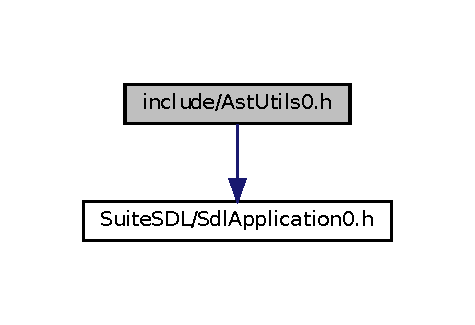
\includegraphics[width=350pt]{AstUtils0_8h__incl}
\end{center}
\end{figure}
\subsection*{Typedefs}
\begin{DoxyCompactItemize}
\item 
using {\bfseries Vector2d} = astu\+::\+Vector2$<$ double $>$
\end{DoxyCompactItemize}
\subsection*{Enumerations}
\begin{DoxyCompactItemize}
\item 
enum \hyperlink{group__error__group_ga59e56af19e754a6aa26a612ebf91d05f}{Error\+Code} \{ \newline
\hyperlink{group__error__group_gga59e56af19e754a6aa26a612ebf91d05fabf350750d0d4fabd8954c0f1e9bbae94}{N\+O\+\_\+\+E\+R\+R\+OR} = 0x0000, 
\hyperlink{group__error__group_gga59e56af19e754a6aa26a612ebf91d05fa0d213a9ce640867b78937ff030c6c76f}{I\+N\+V\+A\+L\+I\+D\+\_\+\+P\+A\+R\+A\+M\+E\+T\+ER}, 
\hyperlink{group__error__group_gga59e56af19e754a6aa26a612ebf91d05face1c457724777c90dbb21eb78cde4ced}{U\+N\+A\+B\+L\+E\+\_\+\+T\+O\+\_\+\+O\+P\+E\+N\+\_\+\+F\+I\+L\+E\+\_\+\+F\+O\+R\+\_\+\+R\+E\+A\+D\+I\+NG}, 
\hyperlink{group__error__group_gga59e56af19e754a6aa26a612ebf91d05faf97c14c5fb1bc0a6b8b19fb96532b7d6}{U\+N\+A\+B\+L\+E\+\_\+\+T\+O\+\_\+\+O\+P\+E\+N\+\_\+\+F\+I\+L\+E\+\_\+\+F\+O\+R\+\_\+\+W\+R\+I\+T\+I\+NG}, 
\newline
\hyperlink{group__error__group_gga59e56af19e754a6aa26a612ebf91d05fa05530b4c73c413c68420467bb3849903}{U\+N\+A\+B\+L\+E\+\_\+\+T\+O\+\_\+\+R\+E\+A\+D\+\_\+\+F\+I\+LE}, 
\hyperlink{group__error__group_gga59e56af19e754a6aa26a612ebf91d05fafc9167af8c15765c886bc48a4812ad57}{U\+N\+A\+B\+L\+E\+\_\+\+T\+O\+\_\+\+I\+M\+P\+O\+R\+T\+\_\+\+F\+I\+LE}, 
\hyperlink{group__error__group_gga59e56af19e754a6aa26a612ebf91d05fa9bf1138c8c1f4519e5b814514b750ca3}{N\+O\+T\+\_\+\+S\+U\+P\+P\+O\+R\+T\+ED}, 
\hyperlink{group__error__group_gga59e56af19e754a6aa26a612ebf91d05fa3a01eacac22f2ede34b2e254ad6c5f6a}{I\+N\+V\+A\+L\+I\+D\+\_\+\+S\+T\+A\+TE}, 
\newline
\hyperlink{group__error__group_gga59e56af19e754a6aa26a612ebf91d05fa8a98e7877e367accbc17e4c1b333a422}{S\+D\+L\+\_\+\+E\+R\+R\+OR}, 
\hyperlink{group__error__group_gga59e56af19e754a6aa26a612ebf91d05fa8dec6f40e00f4411723a80830addf416}{J\+A\+C\+K\+\_\+\+E\+R\+R\+OR}, 
\hyperlink{group__error__group_gga59e56af19e754a6aa26a612ebf91d05fa0a53212262724ecd8005236640d22c96}{A\+P\+P\+\_\+\+E\+R\+R\+OR}, 
\hyperlink{group__error__group_gga59e56af19e754a6aa26a612ebf91d05fa4d17e74c73af4c7b64c944c78d07da2a}{U\+N\+K\+N\+O\+W\+N\+\_\+\+E\+R\+R\+O\+R\+\_\+\+C\+O\+DE}
 \}
\end{DoxyCompactItemize}
\subsection*{Functions}
\begin{DoxyCompactItemize}
\item 
void \hyperlink{group__io__group_ga43fd6e7b7a627ba82ff93795559479f8}{Say\+Hello} ()
\item 
void \hyperlink{group__io__group_gaa8fd8044fbf35d58e73087b6399cd82a}{Say\+Error} ()
\item 
void \hyperlink{group__io__group_ga82cdf45375c3b92b2a60c3d9b55d682f}{Say\+Text} (const char $\ast$text=nullptr, bool eol=true)
\item 
void \hyperlink{group__io__group_gaa78da65e44d9ab5e70c79ed77f62b86a}{Say\+Int} (int value, bool eol=true)
\item 
void \hyperlink{group__io__group_ga6af59270fa536fa4c3e9f8434a8fb4a0}{Say\+Double} (double value, bool eol=true)
\item 
void \hyperlink{group__io__group_gaccd19a10653fad0734fe384cd6d7ba53}{Say\+Version} ()
\item 
void \hyperlink{group__io__group_ga9988545ab3fddd93e05654323cdb1f4b}{Say\+Elapsed\+Time} (const char $\ast$text=nullptr)
\item 
int \hyperlink{group__io__group_gae3d41902eb45488b04016096918d605c}{Ask\+Int} (const char $\ast$text=nullptr)
\item 
double \hyperlink{group__io__group_ga2ecfe90c9b28dec6725b8df1a0013d0d}{Ask\+Double} (const char $\ast$text=nullptr)
\item 
float \hyperlink{group__io__group_ga973515b754711fc89a018ce64f980c74}{Ask\+Float} (const char $\ast$text=nullptr)
\item 
const char $\ast$ \hyperlink{group__io__group_ga89af41351370788f6b9d33fd0bd89d91}{Ask\+String} (const char $\ast$text=nullptr)
\item 
int {\bfseries Open\+File} (const char $\ast$filename, bool open\+For\+Reading=true)
\item 
const char $\ast$ {\bfseries Read\+String} ()
\item 
double {\bfseries Read\+Double} ()
\item 
int {\bfseries Read\+Int} ()
\item 
int {\bfseries Close\+File} ()
\item 
char {\bfseries Read\+Char} ()
\item 
int {\bfseries Skip\+Line} ()
\item 
bool {\bfseries Readable} ()
\item 
bool {\bfseries Compare\+String} (const char $\ast$s1, const char $\ast$s2)
\item 
double \hyperlink{group__math__group_gafdd4eddaf6eadf34406a865e0cf6a30a}{To\+Radians} (double deg)
\item 
double \hyperlink{group__math__group_gab6efcc6e24e777db0fe5e0d0955c2b2d}{To\+Degrees} (double rad)
\item 
int \hyperlink{group__math__group_ga3b74a8d5a155a56580ecd5617cacb4b1}{Minimum} (int a, int b)
\item 
int \hyperlink{group__math__group_gac4c560cadf6af2e052f767eb02d982c0}{Minimum} (int a, int b, int c)
\item 
int {\bfseries Maximum} (int a, int b)
\item 
int {\bfseries Maximum} (int a, int b, int c)
\item 
double \hyperlink{group__math__group_ga298f9ccec14d3ea06c05ccd1e1e062ac}{Get\+Random\+Double} (double min\+Value=0.\+0, double max\+Value=1.\+0)
\item 
int \hyperlink{group__math__group_gab82c25b1da5feec79806fe080becf2c3}{Get\+Random\+Int} (int min\+Value=0, int max\+Value=32767)
\item 
int \hyperlink{group__math__group_ga06bd02ff0de83d2713683574ac288fb3}{Round\+To\+Int} (double value)
\item 
int \hyperlink{group__math__group_gaaf5732ddb11cda2a05f0f978265a114e}{Greatest\+Common\+Divisor} (int a, int b)
\item 
int \hyperlink{group__math__group_ga322fe1f4e7738ff3234fe70d04daeafe}{Lowest\+Common\+Multiple} (int a, int b)
\item 
void \hyperlink{group__math__group_ga9dffb844db4ac8823c6c957448576ed8}{Shuffle} (int $\ast$values, int num\+Values)
\item 
bool \hyperlink{group__math__group_ga1fbbb8c0c7c30db6995b5a4fa82e1754}{Is\+Bit\+Set} (int value, int bit)
\item 
int \hyperlink{group__math__group_ga8c8748fbb1d3e99db79f20fc17d4e63b}{Set\+Bit} (int value, int bit)
\item 
int \hyperlink{group__math__group_ga4ce9c5e2cee3bf609fcfba01c0f8e6a7}{Clear\+Bit} (int value, int bit)
\item 
void \hyperlink{group__timer__group_ga66509b494102a5c28ba6c8be3eab7733}{Start\+Timer} ()
\item 
void \hyperlink{group__timer__group_gaf3619f34a9bc0184b4578e5337069856}{Stop\+Timer} ()
\item 
int \hyperlink{group__timer__group_ga0c820f6552d69b3cdaac23e6b4662d7a}{Get\+Milliseconds} ()
\item 
int \hyperlink{group__audio__group_gaf55add952fe04c4b2758d18db17c8c91}{Write\+Audio} (const char $\ast$filename, float $\ast$data, int size, int sample\+Rate=44100, int channels=1)
\item 
float $\ast$ \hyperlink{group__audio__group_gac361b2470f0258861b9e34deffc8852a}{Read\+Audio} (const char $\ast$filename, int $\ast$size, int $\ast$sample\+Rate, int $\ast$num\+Channels)
\item 
float $\ast$ \hyperlink{group__audio__group_gabf6e39c7686cd89ddc45a0b6be943279}{Extract\+Channel} (float $\ast$data, int size, int num\+Channels, int channel, int $\ast$result\+Size=nullptr)
\item 
float $\ast$ \hyperlink{group__audio__group_ga701f2f439ffe751ed1a5f0b26d23e1c4}{Interleave\+Channels} (float $\ast$ch1\+Data, float $\ast$ch2\+Data, int size, int $\ast$result\+Size=nullptr)
\item 
float $\ast$ \hyperlink{group__audio__group_ga1f60f80cc1589adf04e9b253a5b872b8}{Convert\+Sample\+Rate} (float $\ast$data, int size, int src\+Rate, int dst\+Rate, int $\ast$result\+Size=nullptr)
\item 
int \hyperlink{group__graphics__group_ga8462a895186f3534786c30df8fd9747e}{Create\+Image} (int w, int h)
\item 
void \hyperlink{group__graphics__group_gaf45b0118bad60d88a6c50d841106bc4a}{Clear\+Image} ()
\item 
int \hyperlink{group__graphics__group_ga7a92adcfb955193d1a9e91891cd390e0}{Write\+Image} (const char $\ast$filename)
\item 
void {\bfseries Set\+Draw\+Color} (int r, int g, int b, int a=255)
\item 
void {\bfseries Set\+Clear\+Color} (int r, int g, int b)
\item 
void {\bfseries Draw\+Line} (double x0, double y0, double x1, double y1, double w=1)
\item 
void {\bfseries Draw\+Circle} (double x, double y, double r)
\item 
int \hyperlink{group__error__group_ga10b9a284527af83a44533867b0aff0fc}{Get\+Last\+Error} ()
\item 
void \hyperlink{group__error__group_ga042670233cf17b3bfb1412a37e7dfd59}{Set\+Last\+Error} (int error\+Code)
\item 
bool \hyperlink{group__error__group_ga9f6d63ccb598465866b249cbd6dd06c7}{Has\+Error} ()
\item 
const char $\ast$ \hyperlink{group__error__group_gac785e42215658e0f7127f3690dd8f788}{Get\+Error\+Message} (int error\+Code)
\item 
const char $\ast$ \hyperlink{group__error__group_gac9be83c8ac2a5d80a2be46487c596eab}{Get\+Last\+Error\+Message} ()
\item 
const char $\ast$ \hyperlink{group__error__group_ga8258f5044a56ed71aeed5633fc8341b6}{Get\+Error\+Details} ()
\item 
void \hyperlink{group__error__group_gac4c413604bb98cf7bb6befe53e748b63}{Set\+Error\+Details} (const char $\ast$text)
\end{DoxyCompactItemize}


\subsection{Detailed Description}
This file defines public functions offered by A\+ST utilities A\+P\+I-\/\+Level 0. 


\hypertarget{SdlApplication_8h}{}\section{include/\+Sdl\+Application.h File Reference}
\label{SdlApplication_8h}\index{include/\+Sdl\+Application.\+h@{include/\+Sdl\+Application.\+h}}


This file defines public functions related to S\+D\+L-\/based applications using A\+ST utilities A\+P\+I-\/\+Level 0.  


This graph shows which files directly or indirectly include this file\+:
\nopagebreak
\begin{figure}[H]
\begin{center}
\leavevmode
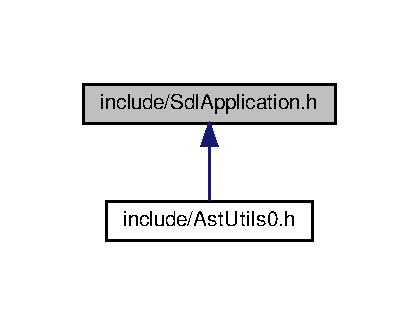
\includegraphics[width=201pt]{SdlApplication_8h__dep__incl}
\end{center}
\end{figure}
\subsection*{Functions}
\begin{DoxyCompactItemize}
\item 
int \hyperlink{group__sdl__group_ga8f43e7993cf196bb0af33a60bc93aa75}{Init\+App} (int width, int height, const char title\mbox{[}$\,$\mbox{]}=\char`\"{}A\+S\+TU/S\+DL Application\char`\"{}, bool vsync=true)
\item 
void \hyperlink{group__sdl__group_gaf4cba1685a7c46bccc7bbdf863114cee}{Quit\+App} ()
\item 
int \hyperlink{group__sdl__group_ga6dfd8bbc85eeeee6922576be9ae65e29}{Set\+Window\+Title} (const char title\mbox{[}$\,$\mbox{]})
\item 
void \hyperlink{group__sdl__group_ga9bf9bfe01e7d336c3a3b13cc923ff850}{Update\+App} ()
\item 
bool \hyperlink{group__sdl__group_ga6d29aa641d22a0299da4710022c8c96b}{Is\+App\+Terminated} ()
\item 
int \hyperlink{group__sdl__group_ga4cc0ada571b47d2b809d441fa6766b52}{Clear\+Canvas} ()
\item 
int \hyperlink{group__sdl__group_gade420aec0a7492d5ac5f320b1ff4a814}{Render\+Line} (double x1, double y1, double x2, double y2)
\item 
int \hyperlink{group__sdl__group_gadd510400a2614b9b8fd8afbe368fc795}{Render\+Point} (double x, double y)
\item 
int \hyperlink{group__sdl__group_gaa5b815a9fcac2b1be46a5957bdbfd13f}{Render\+Rectangle} (double x, double y, double w, double h, bool filled=false)
\item 
int \hyperlink{group__sdl__group_gab01fa8f79d94269a5b9a1cb7d2e51843}{Set\+Render\+Color} (int r, int g, int b, int a=255)
\item 
int \hyperlink{SdlApplication_8h_a56d7cbe37155c107f35dfc13403c6c05}{Set\+Render\+Color} (int argb)
\item 
int \hyperlink{group__sdl__group_ga540012b7df5eddd0b109543deaa66a22}{Set\+Background\+Color} (int r, int g, int b)
\item 
int \hyperlink{SdlApplication_8h_aa80de83a7c03984305662ae0ca5daa05}{Set\+Background\+Color} (int rgb)
\item 
int \hyperlink{group__sdl__group_gaa938d3f784d26ccd4ed8c2d83bbc6ab4}{Get\+Window\+Width} ()
\item 
int \hyperlink{group__sdl__group_gac27ddd893a70056c55278b33d7bd2c62}{Get\+Window\+Height} ()
\item 
int \hyperlink{SdlApplication_8h_a7c508c83150dcd127156d9c4e2436a8e}{Get\+CursorX} ()
\item 
int \hyperlink{SdlApplication_8h_a4769e37502d12fbc431ace1a32749bc8}{Get\+CursorY} ()
\item 
bool \hyperlink{SdlApplication_8h_a2537bad9d6f115fee49a741e7e2623a6}{Is\+Mouse\+Button\+Pressed} (int button)
\item 
double \hyperlink{group__sdl__group_gaf9e3349b29171ad58521f5a7a6238fca}{Get\+Delta\+Time} ()
\item 
double \hyperlink{group__sdl__group_ga9b9387d774c6bc63e5e3c6c91296dedb}{Get\+Absolute\+Time} ()
\item 
void \hyperlink{group__sdl__group_ga5b39467f3664fad21ce3c0f14c4506ff}{Reset\+Absolute\+Time} ()
\item 
double \hyperlink{SdlApplication_8h_aa48ddc248a57dfa1e4afdd6be2a76531}{Get\+Fps} ()
\end{DoxyCompactItemize}


\subsection{Detailed Description}
This file defines public functions related to S\+D\+L-\/based applications using A\+ST utilities A\+P\+I-\/\+Level 0. 



\subsection{Function Documentation}
\mbox{\Hypertarget{SdlApplication_8h_a7c508c83150dcd127156d9c4e2436a8e}\label{SdlApplication_8h_a7c508c83150dcd127156d9c4e2436a8e}} 
\index{Sdl\+Application.\+h@{Sdl\+Application.\+h}!Get\+CursorX@{Get\+CursorX}}
\index{Get\+CursorX@{Get\+CursorX}!Sdl\+Application.\+h@{Sdl\+Application.\+h}}
\subsubsection{\texorpdfstring{Get\+Cursor\+X()}{GetCursorX()}}
{\footnotesize\ttfamily int Get\+CursorX (\begin{DoxyParamCaption}{ }\end{DoxyParamCaption})}

Returns the x-\/coordinate of the mouse cursor.

\begin{DoxyReturn}{Returns}
the x-\/coordinate of the mouse cursor 
\end{DoxyReturn}
\mbox{\Hypertarget{SdlApplication_8h_a4769e37502d12fbc431ace1a32749bc8}\label{SdlApplication_8h_a4769e37502d12fbc431ace1a32749bc8}} 
\index{Sdl\+Application.\+h@{Sdl\+Application.\+h}!Get\+CursorY@{Get\+CursorY}}
\index{Get\+CursorY@{Get\+CursorY}!Sdl\+Application.\+h@{Sdl\+Application.\+h}}
\subsubsection{\texorpdfstring{Get\+Cursor\+Y()}{GetCursorY()}}
{\footnotesize\ttfamily int Get\+CursorY (\begin{DoxyParamCaption}{ }\end{DoxyParamCaption})}

Returns the y-\/coordinate of the mouse cursor.

\begin{DoxyReturn}{Returns}
the y-\/coordinate of the mouse cursor 
\end{DoxyReturn}
\mbox{\Hypertarget{SdlApplication_8h_aa48ddc248a57dfa1e4afdd6be2a76531}\label{SdlApplication_8h_aa48ddc248a57dfa1e4afdd6be2a76531}} 
\index{Sdl\+Application.\+h@{Sdl\+Application.\+h}!Get\+Fps@{Get\+Fps}}
\index{Get\+Fps@{Get\+Fps}!Sdl\+Application.\+h@{Sdl\+Application.\+h}}
\subsubsection{\texorpdfstring{Get\+Fps()}{GetFps()}}
{\footnotesize\ttfamily double Get\+Fps (\begin{DoxyParamCaption}{ }\end{DoxyParamCaption})}

Returns the average frames per seconds (F\+PS).

\begin{DoxyReturn}{Returns}
the frames per seconds 
\end{DoxyReturn}
\mbox{\Hypertarget{SdlApplication_8h_a2537bad9d6f115fee49a741e7e2623a6}\label{SdlApplication_8h_a2537bad9d6f115fee49a741e7e2623a6}} 
\index{Sdl\+Application.\+h@{Sdl\+Application.\+h}!Is\+Mouse\+Button\+Pressed@{Is\+Mouse\+Button\+Pressed}}
\index{Is\+Mouse\+Button\+Pressed@{Is\+Mouse\+Button\+Pressed}!Sdl\+Application.\+h@{Sdl\+Application.\+h}}
\subsubsection{\texorpdfstring{Is\+Mouse\+Button\+Pressed()}{IsMouseButtonPressed()}}
{\footnotesize\ttfamily bool Is\+Mouse\+Button\+Pressed (\begin{DoxyParamCaption}\item[{int}]{button }\end{DoxyParamCaption})}

Tests whether a certain mouse button is currently pressed.


\begin{DoxyParams}{Parameters}
{\em button} & the index of the button to be queried \\
\hline
\end{DoxyParams}
\begin{DoxyReturn}{Returns}
{\ttfamily true} if the mouse button is pressed 
\end{DoxyReturn}
\mbox{\Hypertarget{SdlApplication_8h_aa80de83a7c03984305662ae0ca5daa05}\label{SdlApplication_8h_aa80de83a7c03984305662ae0ca5daa05}} 
\index{Sdl\+Application.\+h@{Sdl\+Application.\+h}!Set\+Background\+Color@{Set\+Background\+Color}}
\index{Set\+Background\+Color@{Set\+Background\+Color}!Sdl\+Application.\+h@{Sdl\+Application.\+h}}
\subsubsection{\texorpdfstring{Set\+Background\+Color()}{SetBackgroundColor()}}
{\footnotesize\ttfamily int Set\+Background\+Color (\begin{DoxyParamCaption}\item[{int}]{rgb }\end{DoxyParamCaption})}

Sets the background color of the application window.

The background color does not have an alpha channel and cannot be transparent.

This function can be used to set the background color using the usual hex-\/triplet notation which is a six-\/digit, three-\/byte hexadecimal number used int H\+T\+ML, C\+SS, S\+VG etc. \mbox{\Hypertarget{SdlApplication_8h_a56d7cbe37155c107f35dfc13403c6c05}\label{SdlApplication_8h_a56d7cbe37155c107f35dfc13403c6c05}} 
\index{Sdl\+Application.\+h@{Sdl\+Application.\+h}!Set\+Render\+Color@{Set\+Render\+Color}}
\index{Set\+Render\+Color@{Set\+Render\+Color}!Sdl\+Application.\+h@{Sdl\+Application.\+h}}
\subsubsection{\texorpdfstring{Set\+Render\+Color()}{SetRenderColor()}}
{\footnotesize\ttfamily int Set\+Render\+Color (\begin{DoxyParamCaption}\item[{int}]{argb }\end{DoxyParamCaption})}

Sets the render color for subsequent render calls.
\begin{DoxyItemize}
\item This function can be used to set the background color using the usual hex-\/triplet notation which is a six-\/digit, three-\/byte hexadecimal number used int H\+T\+ML, C\+SS, S\+VG etc.
\end{DoxyItemize}

{\bfseries Example Usage}


\begin{DoxyCode}
\textcolor{comment}{// Set render color to orange, full opaque.}
\hyperlink{group__sdl__group_gab01fa8f79d94269a5b9a1cb7d2e51843}{SetRenderColor}(0xFFFFA500);

\textcolor{comment}{// Set render color to yellow, 50% transparent.}
\hyperlink{group__sdl__group_gab01fa8f79d94269a5b9a1cb7d2e51843}{SetRenderColor}(0x80ffff00);

\textcolor{comment}{// Set render color to white, full opaque.}
\hyperlink{group__sdl__group_gab01fa8f79d94269a5b9a1cb7d2e51843}{SetRenderColor}(0xffffffff);
\end{DoxyCode}
 
%--- End generated contents ---

% Index
\backmatter
\newpage
\phantomsection
\clearemptydoublepage
\addcontentsline{toc}{chapter}{Index}
\printindex

\end{document}
